% !TEX root = handbook-physics.tex
% !TEX TS-program = pdflatex
% !TEX encoding = UTF-8 Unicode




\chapter[Properties Of Atomic Nuclei]{Structure And Basic Properties Of Atomic Nuclei}
\label{ch-42}
\zhtitle{原子核的结构与基本性质}

\section{Main Properties and Structure of the Nucleus}
\label{sec-42.1} 
\zhtitle{原子核的主要性质与结构}

\subsection{}\label{42.1.1} 

The \redem{nucleus} is the central part of an atom; practically all of the atom's mass and its positive charge are concentrated in the nucleus. All atomic nuclei are made up of elementary particles \ssect{43.1.1} called \redem{protons} and \redem{neutrons}, considered to be
two charge states of a single particle called the nucleon. The proton has a positive electric charge, equal in magnitude to that of the electron \ssect{14.1.2}. The neutron has no electric charge.
\zhpar{\redem{原子核}是原子的中心部分；原子的几乎全部质量和全部正电荷都集中在原子核中。所有原子核都由基本粒子\ssect{43.1.1}组成，这些粒子称为\redem{质子}和\redem{中子}，它们被看作同一种粒子——核子——的两种电荷状态。质子带正电，其电荷量的绝对值与电子相同\ssect{14.1.2}；中子不带电。}

\subsection{}\label{42.1.2} 

The \redem{charge of the nucleus} is the quantity $Z_{e}$, where $e$ is the electron charge, and $Z$ is the atomic number of the chemical element in Mendeleev's periodic table \ssect{39.3.5} and is equal to the number of protons in the nucleus. Up to date nuclei are known with $Z$ ranging from $Z = 1$ to $Z = 107$. For all nuclei, with the exception of \ce{^{1}_{1}H}, \ce{^{3}_{1}He} and certain other neutron-deficient nuclei, $N \geqslant  Z$, where $N$ is the number of neutrons in the nucleus. For light nuclei $N/Z \approx 1$; for the nuclei of chemical elements at the end of the periodic system, $N/Z \approx 1.6$.
\zhpar{\redem{原子核的电荷}为 $Z_{e}$，其中 $e$ 为电子电荷，$Z$ 为化学元素在门捷列夫周期表中的原子序数\ssect{39.3.5}，它等于原子核中的质子数。迄今已知的原子核，其 $Z$ 值从 $Z = 1$ 到 $Z = 107$。除 \ce{^{1}_{1}H}、\ce{^{3}_{1}He} 以及其他某些缺中子核外，所有原子核都满足 $N \geqslant  Z$，其中 $N$ 为原子核中的中子数。轻核的 $N/Z \approx 1$；周期表末端化学元素的原子核，$N/Z \approx 1.6$。}

\subsection{}\label{42.1.3} 

The number of nucleons \ssect{42.1.1} in a nucleus, $A = N 
+ Z$, is called the \redem{mass}, or \redem{nucleon, number}. Nucleons (proton and neutron) are assigned a mass number equal to unity. The electron has zero mass number.
\zhpar{原子核中的核子数 \ssect{42.1.1} $A = N + Z$ 称为\redem{质量数}，或\redem{核子数}。核子（质子和中子）的质量数规定为 1，电子的质量数为零。}

Nuclei with the same $Z$ value, but different $A$ values are called \redem{isotopes}. Nuclei with the same $A$ value, but different $Z$ values are called \redem{isobars}. The nucleus of chemical element $X$ is denoted by the symbol $^{A}_{Z}X$, where $X$ is the symbol of the chemical element.
\zhpar{具有相同 $Z$ 值而 $A$ 值不同的原子核称为\redem{同位素}；具有相同 $A$ 值而 $Z$ 值不同的原子核称为\redem{同量异位素}。化学元素 $X$ 的原子核用符号 $^{A}_{Z}X$ 表示，其中 $X$ 为该化学元素的符号。}

About 300 stable isotopes of chemical elements are found in
nature, and there are over a 1000 man-made (radioactive)
isotopes.
\zhpar{自然界中存在约 300 种稳定的化学元素同位素，而人工（放射性）同位素则超过 1000 种。}

\subsection{}\label{42.1.4} 

The size of a nucleus is specified by Lite \redem{nuclear radius} $r$, which has only an arbitrary meaning because the nucleus has no clearly defined boundary. The empirical formula for the nuclear radius is $r = r_{0}A^{1/3}$, where $r_{0} = (1.3 \text{ to } 1.7) \SI{d-16}{\meter}$ can be interpreted as the proportionality of the volume of the nucleus to the number of nucleons it contains.
\zhpar{原子核的大小由\redem{原子核半径} $r$ 来描述，但它只有任意的意义，因为原子核并没有明确的边界。原子核半径的经验公式为 $r = r_{0}A^{1/3}$，其中 $r_{0} = (1.3 \text{ to } 1.7) \SI{d-16}{\meter}$，这一关系可以理解为原子核的体积与其所含核子数成正比。}

The density of nuclear matter is of the order of magnitude of \SI{d17}{\kilo\gram\per\meter\cubed} and is constant for all nuclei. It substantially exceeds the density of the most dense of ordinary substances.
\zhpar{核物质的密度约为 \SI{d17}{\kilo\gram\per\meter\cubed} 量级，且对所有原子核都相同。它远大于最致密的普通物质的密度。}

\subsection{}\label{42.1.5} Nucleons in atomic nuclei are fermions \ssect{41.2.4} and their spin equals $\hbar /2$. The nucleus of an atom has intrinsic angular momentum, called \redem{nuclear spin}, equal to $L_{N} =
= \sqrt{ I(I+1)} \hbar$, where $I$ is the \redem{inner (total) spin quantum number} (cf. \ssect{26.1.3}), $\hbar = h/2 \pi$ and $h$ is Planck's constant (Appendix~II). 
\zhpar{原子核中的核子是费米子\ssect{41.2.4}，其自旋为 $\hbar /2$。原子核具有内禀角动量，称为\redem{核自旋}，其大小为 $L_{N} = \sqrt{ I(I+1)} \hbar$，其中 $I$ 为\redem{内（总）自旋量子数}（参见\ssect{26.1.3}），$\hbar = h/2 \pi$，$h$ 为普朗克常量（见附录 II）。}

The number $I$ may assume any whole or half-integer value:
0, 1/2, 1, 3/2, 2, etc. Nuclei with even mass numbers Adiavc
integer spin (in $\hbar$ units) and comply with Bose-Einstein'statistics \ssect{41.2.1}. Nuclei with odd mass numbers $A$ have half integer spin (in $\hbar$ units) and comply with Fermi-Dirac statistics \ssect{41.2.4}.
\zhpar{自旋量子数 $I$ 可取任意的整数或半整数：0, 1/2, 1, 3/2, 2 等。质量数为偶数的原子核，其自旋为整数（以 $\hbar$ 为单位），服从玻色-爱因斯坦统计\ssect{41.2.1}；质量数 $A$ 为奇数的原子核，其自旋为半整数（以 $\hbar$ 为单位），服从费米-狄拉克统计\ssect{41.2.4}。}

\subsection{}\label{42.1.6}


Nuclear particles have their intrinsic magnetic moments,
which determine the \redem{total nuclear magnetic moment} $P_{mN}$. The unit of measurement of nuclear magnetic moments is the \redem{nuclear magneton} $\mu_{N}$ analogous to Bohr's magneton \ssect{26.1.4}. Thus
\zhpar{核粒子具有各自的固有磁矩，它们共同决定了\redem{原子核的总磁矩} $P_{mN}$。核磁矩的度量单位为\redem{核磁子} $\mu_{N}$，它类似于玻尔磁子\ssect{26.1.4}。于是有}
\begin{align*}%
\mu_{N} & = \frac{e \hbar}{2 m_{p}} && \text{(in SI units),}\\
\mu_{N} & = \frac{e \hbar}{2 m_{p}c} && \text{(in Gaussian units),}
\end{align*}
where $e$ is the magnitude of the electron charge, $m_{p}$ is the mass of the proton, and $c$ is the electrodynamic constant (Appendix~II).
\zhpar{式中 $e$ 为电子电荷的大小，$m_{p}$ 为质子的质量，$c$ 为电动力学常量（见附录 II）。}

The nuclear magneton is a factor $m_{p}/m_{e} = 1836.5$ times less than the Bohr magneton. It follows that the magnetic properties of atoms are determined by those of their electrons.
\zhpar{核磁子比玻尔磁子小 $m_{p}/m_{e} = 1836.5$ 倍。因此，原子的磁性质由其电子的磁性质决定。}

The following relation exists between nuclear spin $L_{N}$, measured in $\hbar$ units, and the magnetic moment of the  ucleus, measured in nuclear magnetons:
\zhpar{以 $\hbar$ 为单位度量的核自旋 $L_{N}$，与以核磁子为单位度量的原子核磁矩之间，存在如下关系：}
\begin{equation*}%
P_{mN} = \gamma_{N} L_{N},
\end{equation*}
where $\gamma_{N}$ is the \redem{nuclear gyromagnelic ratio} (cf. \ssect{26.1.4}).
\zhpar{其中 $\gamma_{N}$ 为\redem{核旋磁比}（参见\ssect{26.1.4}）。}

The magnetic moments of the neutron and proton are associated with their complex internal structure \ssect{43.6.2}. The neutron has a negative magnetic moment equal to $-(1.91314 \pm 0.00005) \mu_{N}$. The spin of the neutron and its magnetic moment are opposite in direction. The magnetic moment of the proton is positive and is equal to $(2.79277 \pm 0.00003) \mu_{N}$. Its direction coincides with the direction of proton spin.
\zhpar{中子和质子的磁矩与其复杂的内部结构有关\ssect{43.6.2}。中子具有负磁矩，其值为 $-(1.91314 \pm 0.00005) \mu_{N}$，中子的自旋与其磁矩方向相反。质子的磁矩为正，其值为 $(2.79277 \pm 0.00003) \mu_{N}$，其方向与质子自旋的方向一致。}


\subsection{}\label{42.1.7}

In the general case, the distribution of electric charge
of the proton in the nucleus is asymmetrical. A measure of the deviation of this distribution from spherical symmetry is the \redem{electric quadrupole moment of the nucleus} $Q$. If the charge density is assumed the same throughout the nucleus, $Q$ is determined only by the shape of the nucleus. For an ellipsoid of revolution
\zhpar{一般情况下，原子核中电荷的分布是不对称的。度量这种分布偏离球对称程度的物理量是原子核的\redem{电四极矩} $Q$。若假定整个原子核内的电荷密度相同，则 $Q$ 仅由原子核的形状决定。对于旋转椭球体，有}
\begin{equation*}%
Q = \frac{2}{5} Z_{e} (b^{2} - a^{2}),
\end{equation*}
where $b$ is the semiaxis of the ellipsoid along its spin, and $a$ is the semiaxis in the perpendicular direction. For a nucleus stretched out along its spin, $b > a$ and $Q > 0$. For a nucleus flattened in this direction, $b < a$ and $Q < 0$. For spherical distribution of the charge in the nucleus, $b = a$ and $Q = 0$. This is valid for nuclei with spin equal to 0 or to $(1/2) \hbar$.
\zhpar{式中 $b$ 为椭球沿自旋方向的半轴，$a$ 为垂直于该方向的半轴。对于沿自旋方向拉长的原子核，$b > a$，$Q > 0$；对于沿此方向压扁的原子核，$b < a$，$Q < 0$。若电荷在原子核中呈球对称分布，则 $b = a$，$Q = 0$。这一结论适用于自旋为 0 或 $(1/2) \hbar$ 的原子核。}

\section{Binding Energy of Nuclei. Mass Defect}
\label{sec-42.2} 
\zhtitle{原子核的结合能。质量亏损}

\subsection{}\label{42.2.1} 

In nuclei, nucleons are in states that differ essentially
from their free states. With the exception of the nucleus of ordinary hydrogen, all nuclei contain at least two nucleons, between which there exists a special \redem{nuclear strong interaction} --- attraction --- that ensures stability of the nucleus notwithstanding the repulsion of the protons of like charge.
\zhpar{在原子核中，核子所处的状态与其自由状态有本质区别。除普通氢的原子核外，所有原子核都至少包含两个核子，核子之间存在一种特殊的\redem{核强相互作用}——吸引力，它保证了原子核的稳定性，抵消了同种电荷质子之间的斥力。}


\subsection{}\label{42.2.2}

The \redem{binding energy of a nucleon} in a nucleus is the physical quantity equal to the work required to remove the nucleon from the nucleus without imparting kinetic energy to it. 
\zhpar{\redem{核子在原子核中的结合能}是指将核子从原子核中移出、且不使其获得动能所需做的功，它是一个物理量。}

The \redem{nuclear binding energy} is the amount of work required to take the nucleus apart into its component nucleons without imparting any kinetic energy to them. It follows from the law of energy conservation that in forming a nucleus the same amount of energy is released as is required in splitting the nucleus into its component nucleons. The nuclear binding energy is the difference between the total energy of all the free nucleons that make up the nucleus and their total energy in the nucleus.
\zhpar{\redem{原子核的结合能}是指将原子核拆散为各组成核子、且不使核子获得任何动能所需做的功。由能量守恒定律可知，形成原子核时释放的能量与将原子核拆分为组成核子所需的能量相等。原子核的结合能等于组成该核的所有自由核子的总能量与它们在原子核中的总能量之差。}

\subsection{}\label{42.2.3}

In forming a nucleus, its mass is reduced: the mass of the
nucleus is less than the total mass of its component nucleons. This reduction in mass in the formation of a nucleus is due, to the release of the binding energy. If $\Delta E_{b}$ is the amount of energy released in forming a nucleus, the corresponding mass $\Delta m$ \ssect{5.7.6}, equal to 
\zhpar{形成原子核时，其质量减少：原子核的质量小于组成它的核子的总质量。原子核形成时的这种质量减少，是由于释放了结合能。若 $\Delta E_{b}$ 为形成原子核时释放的能量，则与之对应的质量 $\Delta m$ \ssect{5.7.6} 为}
\begin{equation*}%
\Delta m = \frac{\Delta E_{b}}{c^{2}},
\end{equation*}
is called the \redem{mass defect} and characterizes the reduction in the total mass in forming a nucleus from its component nucleons. 
\zhpar{该质量 $\Delta m$ 称为\redem{质量亏损}，它表征了由组成核子形成原子核时总质量的减少。}

If a nucleus of mass $m_{N}$ is formed of $Z$ protons with the mass $m_{p}$ and of $(A - Z)$ neutrons of mass then
\zhpar{若质量为 $m_{N}$ 的原子核由 $Z$ 个质量为 $m_{p}$ 的质子和 $(A - Z)$ 个质量为 $m_{n}$ 的中子组成，则}
\begin{equation*}%
\Delta m = Z m_{p} + (A- Z) m_{n} - m_{N}.
\end{equation*}
Instead of the mass $m_{N}$ of the nucleus, the quantity $\Delta m$ can he expressed in terms of the atomic mass $m_{a}$. Thus
\zhpar{也可以用原子质量 $m_{a}$ 代替原子核质量 $m_{N}$ 来表示 $\Delta m$。于是有}
\begin{equation*}%
\Delta m = Z m_{H} + (A- Z) m_{n} - m_{a}.
\end{equation*}
where $m_{H}$ is the mass of the hydrogen atom.
\zhpar{式中 $m_{H}$ 为氢原子的质量。}

In practice, in calculating $\Delta m$, the masses of all the particles and atoms are expressed in atomic mass units (Appendix~II). The mass defect serves as a measure of the nuclear binding energy. Thus
\zhpar{计算 $\Delta m$ 时，所有粒子和原子的质量都以原子质量单位表示（见附录 II）。质量亏损可用来度量原子核的结合能。于是有}
\begin{equation*}%
\Delta E_{b} = \Delta mc^{2} = [Z m_{p} + (A - Z)m_{n} - m_{N}]c^{2}.
\end{equation*}
One atomic mass unit corresponds to \redem{one atomic unit of energy}, which is equal to \SI{931.5016}{\mega\electronvolt}.
\zhpar{一个原子质量单位相当于\redem{一个原子能量单位}，其值等于 \SI{931.5016}{\mega\electronvolt}。}


\subsection{}\label{42.2.4}

The \redem{specific binding energy} $\Delta E^{nu}_{b}$ of the nucleus is the binding energy per nucleon: $\Delta E^{nu}_{b} = \Delta E_{b}/A$. The quantity $\Delta E^{nu}_{b}$ equals \SI{8}{\mega\electronvolt}/nucleon on an average. A curve showing the dependence of the specific binding energy on the mass number $A$ and characterizing the different bonding strengths for the nucleons in the nuclei of various chemical elements, is given in \figr{fig-42-01}. The nuclei of elements in the middle of the periodic system \ssect{39.3.5} $(28 < A < 138)$, i.e. from \ce{^{28}_{14}Si} to \ce{^{138}_{56}Ba} have the strongest bonds. In these nuclei $\Delta E^{nu}_{b}$ is close to \SI{8.7}{\mega\electronvolt}/nucleon. 
\zhpar{原子核的\redem{比结合能} $\Delta E^{nu}_{b}$ 是每个核子的结合能：$\Delta E^{nu}_{b} = \Delta E_{b}/A$。$\Delta E^{nu}_{b}$ 的平均值约为 \SI{8}{\mega\electronvolt}/核子。\figr{fig-42-01}给出了比结合能随质量数 $A$ 变化的曲线，它表征了不同化学元素的原子核中核子的不同结合强度。位于周期表中部的元素的原子核（$28 < A < 138$），即从 \ce{^{28}_{14}Si} 到 \ce{^{138}_{56}Ba}，其结合最为紧密。在这些原子核中，$\Delta E^{nu}_{b}$ 接近 \SI{8.7}{\mega\electronvolt}/核子。}

As the number of nucleons in the nucleus
increases, the specific binding energy decreases. The atomic
nuclei of chemical elements located at the end of the periodic system (for instanc, the nucleus of uranium) have the binding energy \SI{7.6}{\mega\electronvolt}/nucleon. This explains the feasibility of releasing energy by the fission of heavy nuclei \ssect{42.9.2}. In the region of low mass numbers there are sharp peaks of specific binding energy. Maxima are typical for nuclei with even numbers of protons and neutrons (\ce{^{4}_{2}He}, \ce{^{12}_{6}C}, \ce{^{16}_{8}O}). Minima are typical for nuclei with odd numbers of protons and neutrons (\ce{_{3}Li}, \ce{_{5}B}, \ce{_{7}N}).
\zhpar{随着原子核中核子数的增加，比结合能减小。位于周期表末端的化学元素的原子核（例如铀核），其结合能仅为 \SI{7.6}{\mega\electronvolt}/核子。这说明了重核裂变时可以释放能量的原因\ssect{42.9.2}。在低质量数区域，比结合能有尖锐的峰值。偶数质子数与偶数中子数的原子核（\ce{^{4}_{2}He}、\ce{^{12}_{6}C}、\ce{^{16}_{8}O}）呈现极大值；奇数质子数与奇数中子数的原子核（\ce{_{3}Li}、\ce{_{5}B}、\ce{_{7}N}）呈现极小值。}

\begin{figure}%[-3cm] 
\centering
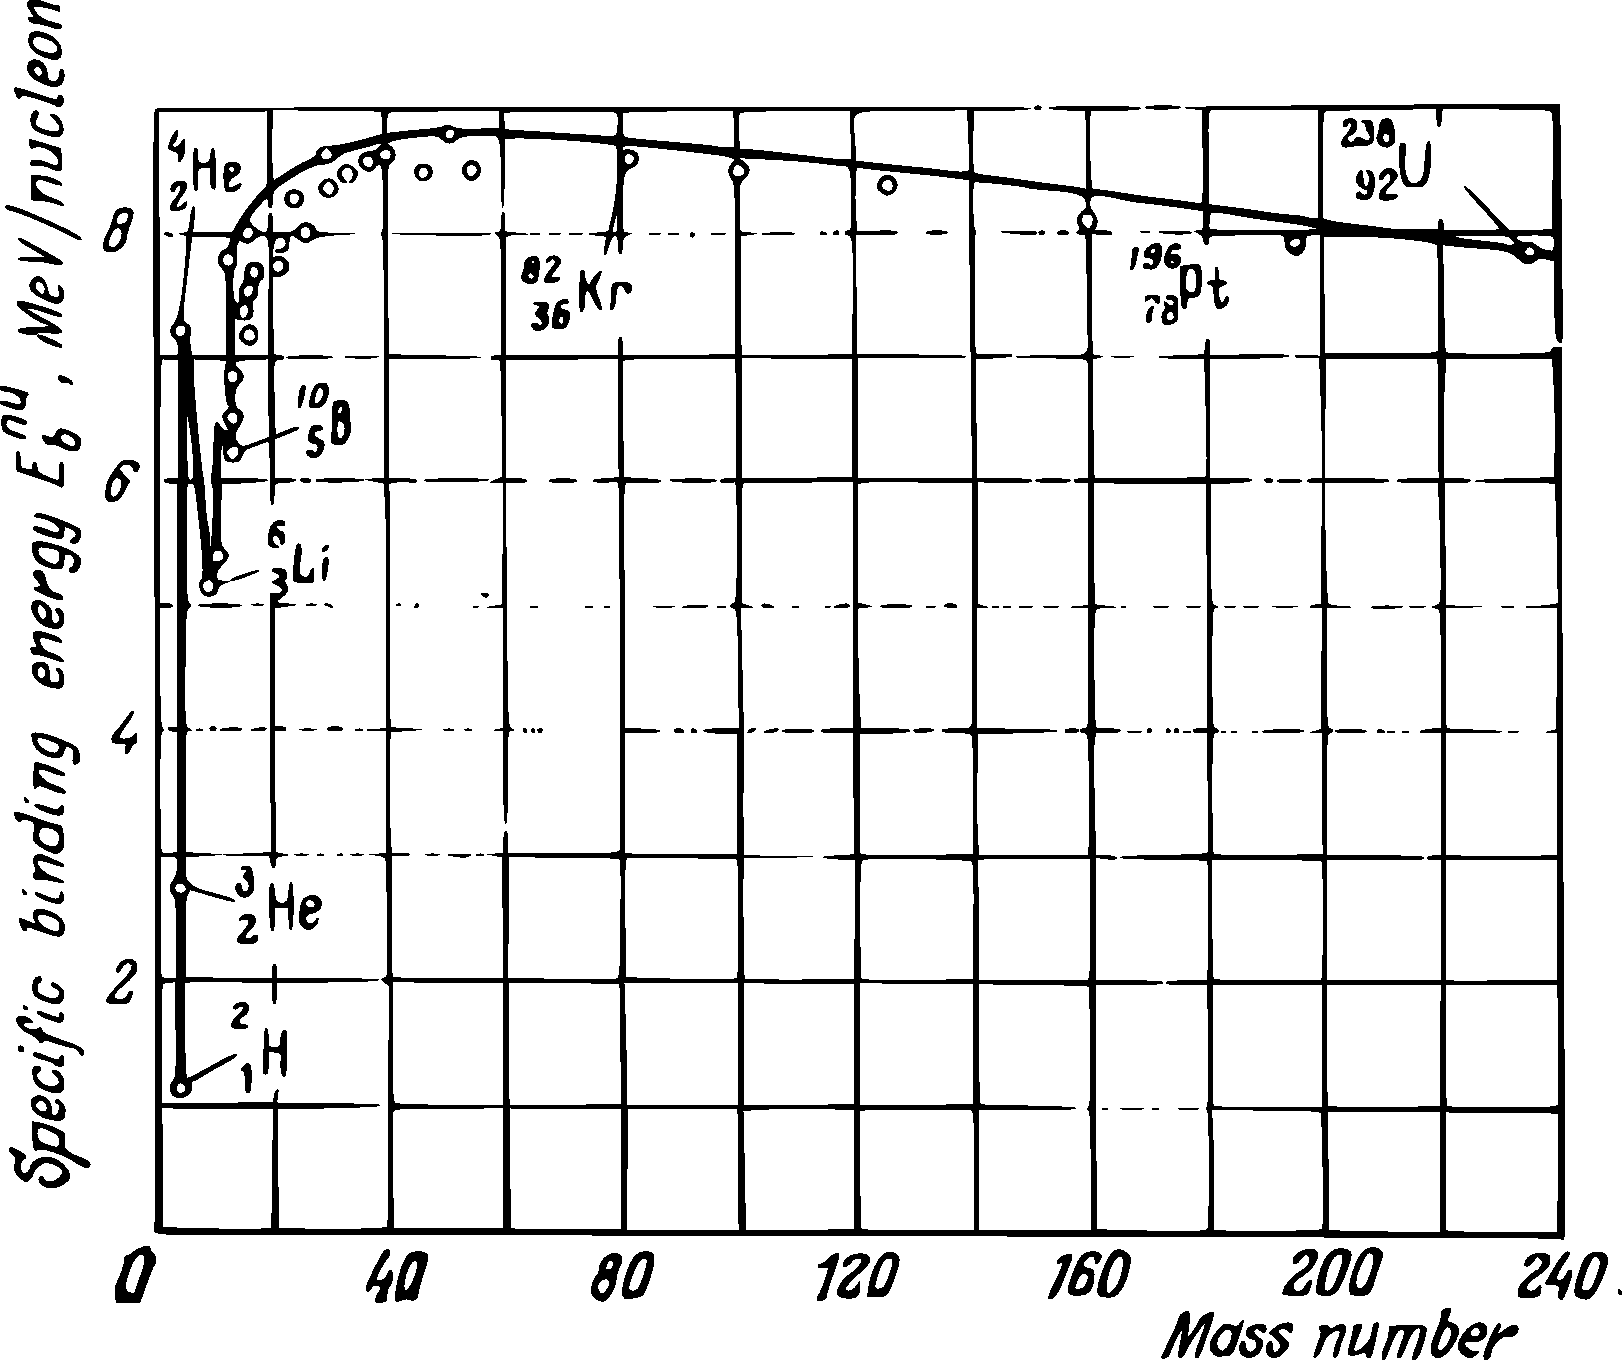
\includegraphics[width=\textwidth]{figs/ch-42/fig-42-01.pdf}
\sidecaption{The dependence of the specific binding energy on the mass number $A$.\zhcap{比结合能随质量数 $A$ 的变化关系。}\label{fig-42-01}}
\end{figure}

\subsection{}\label{42.2.5} Data on the binding energy of the nucleus and an application of the liquid-drop model of the nucleus\sidenote{The liquid-drop model of the nucleus is discussed in the physics course of secondary schools.} enabled certain laws of nuclear structure to be established.
\zhpar{原子核结合能的数据，以及原子核液滴模型的应用，使人们得以建立原子核结构的若干规律。}
\zhpar{注：原子核的液滴模型在中学物理课程中已有介绍。}



The \redem{atomic nuclear stability criterion} is the relation between the numbers of protons and neutrons in a stable nucleus for the given isobars \ssect{42.1.3} (i.e. $A = \text{ const})$. The condition for minimum energy of the nucleus yields the following relation between $Z_{st}$ and $A$:
\zhpar{\redem{原子核稳定性判据}是指：对于给定的同量异位素（即 $A = \text{const}$），稳定原子核中质子数与中子数之间的关系。原子核能量取极小值的条件给出 $Z_{st}$ 与 $A$ 之间如下的关系：}
\begin{equation*}%
Z_{st} = \frac{A}{ 1.98 + 0.015A^{2/3}}.
\end{equation*}
The stable atomic numbers $Z_{st}$ are the nearest whole numbers to those obtained by this formula. 
\zhpar{由该公式算出的数值中，最接近的整数即为稳定原子序数 $Z_{st}$。}

At low and medium values of $A$ there are approximately equal numbers of protons and neutrons in stable nuclei: $N \approx Z$ or $A \approx 2Z$. Especially stable are nuclei (when $Z = A/2$) for which $N$ or $Z = 2$, 8, 20, 28, 50, 82 or 126. These have been called \redem{magic numbers}. Nuclei in which both $N$ and $Z$ are magic numbers are said to be \redem{double-magic}.
\zhpar{在 $A$ 值较小和中等时，稳定原子核中质子数与中子数大致相等：$N \approx Z$，或 $A \approx 2Z$。特别稳定的原子核（$Z = A/2$ 时）满足 $N$ 或 $Z = 2$、8、20、28、50、82 或 126。这些数被称为\redem{幻数}。$N$ 与 $Z$ 均为幻数的原子核称为\redem{双幻核}。}

As $Z$ increases, the Coulomb forces of repulsion between the protons increases in proportion to $Z (Z - 1) \approx Z^{2}$ (pairwise proton interaction), and, to compensate for this repulsion by nuclear attraction, the number of neutrons must increase more rapidly than the number of protons.
\zhpar{随着 $Z$ 增大，质子之间的库仑斥力按 $Z (Z - 1) \approx Z^{2}$ 的比例增长（质子两两相互作用），为了用核的吸引力补偿这种斥力，中子数必须比质子数增加得更快。}

\section{Nuclear Forces}
\label{sec-42.3} 
\zhtitle{核力}

\subsection{}\label{42.3.1} 

Nuclear interaction indicates that special \redem{forces exist in nuclei} that do not belong to any of the types of forces known in classical physics (e.g. gravitational and electromagnetic forces).
\zhpar{核相互作用表明，原子核中存在\redem{特殊的力}，它不属于经典物理学中已知的任何一类力（例如引力和电磁力）。}

\subsection{}\label{42.3.2}

Nuclear forces are of short-range action. They only act
at the extremely short distances, of the order of \SI{d-15}{\meter}, between nucleons in a nucleus. This distance, ranging from 1.5 to \SI{2.2d-15}{\meter}, is called the \redem{action radius}, or \redem{range, of the nuclear forces}.
\zhpar{核力是短程力。它只在原子核中核子之间极短的距离上起作用，该距离约为 \SI{d-15}{\meter} 量级。这一距离在 1.5 至 \SI{2.2d-15}{\meter} 之间，称为\redem{作用半径}，或称核力的\redem{力程}。}

\subsection{}\label{42.3.3}

Nuclear forces display \redem{charge independence}: the attraction between any two nucleons is the same and is independent of the charge state of the nucleons, regardless of whether they are protons or neutrons \sect{42.1.1}. The charge independence of nuclear forces follows from a comparison of the binding energy in \redem{mirror nuclei}. These are nuclei having the same total number of nucleons, but the number of protons in one is equal to the number of neutrons in the other. The nuclei of helium \ce{^{3}_{2}He} and tritium \ce{^{3}_{1}T} (superheavy hydrogen) can be taken as an example.
\zhpar{核力具有\redem{电荷无关性}：任意两个核子之间的吸引力都相同，与核子的电荷状态无关，无论它们是质子还是中子\sect{42.1.1}。核力的电荷无关性可由\redem{镜像核}的结合能比较得出。镜像核是指核子总数相同、但其中一个核的质子数等于另一个核的中子数的原子核。氦-3 \ce{^{3}_{2}He} 与氚 \ce{^{3}_{1}T}（超重氢）即为一例。}

The binding energies \sect{42.2.4} in these nuclei are \SI{7.72}{\mega\electronvolt} and \SI{8.49}{\mega\electronvolt}, respectively. Assuming charge independence of nuclear forces, the difference in the nuclear binding energies, equal to \SI{0.77}{\mega\electronvolt}, is associated with the energy of Coulomb repulsion between two protons in the nucleus of \ce{^{3}_{2}He}. Assuming this quantity equal to $e^{2}/4\pi \varepsilon_{0}r$ \sect{16.2.6}, the average distance $r$ between
the protons in the \ce{^{3}_{2}He} nucleus is found to equal \SI{1.9d-15}{\meter}. This is in agreement with the action radius of nuclear forces \sect{42.3.2}.
\zhpar{这两个原子核的结合能分别为 \SI{7.72}{\mega\electronvolt}（\ce{^{3}_{2}He}）和 \SI{8.49}{\mega\electronvolt}（\ce{^{3}_{1}T}）。假定核力具有电荷无关性，两者结合能之差 \SI{0.77}{\mega\electronvolt} 应归因于 \ce{^{3}_{2}He} 核中两个质子之间的库仑斥能。取该能量等于 $e^{2}/4\pi \varepsilon_{0}r$\sect{16.2.6}，可求得 \ce{^{3}_{2}He} 核中质子之间的平均距离 $r$ 约为 \SI{1.9d-15}{\meter}。这与核力的作用半径相符\sect{42.3.2}。}

\subsection{}\label{42.3.4}

Nuclear forces have the property of \redem{saturation}. This
is manifested in the fact that a nucleon in the nucleus interacts with only a limited number of the closest nucleons among its neighbours. Besides the short-range action of nuclear forces \sect{42.3.1}, this saturation also follows from the linear dependence of the binding energy in nuclei on the mass number $A$ \sect{42.1.3}.
\zhpar{核力具有\redem{饱和性}。这表现为：原子核中的一个核子只与其邻近的、数目有限的最近核子发生相互作用。除核力的短程作用\sect{42.3.1}外，这种饱和性还可由原子核的结合能与质量数 $A$ 呈线性关系得出\sect{42.1.3}。}

If each nucleon in a nucleus interacted simultaneously with
all $(A - 1)$ nucleons in the nucleus, the binding energy of the nucleus would be proportional to the possible number of interacting pairs of nucleons in the nucleus, i.e. the number of combinations of $A$ taken two at a time: $A (A - 1)/2$.\sidenote{Assuming, of course, pairwise nuclear interaction.} The dependence, in this case, of the binding energy on $A$ would be quadratic, rather than linear, and this is in contradiction with the experimental data. Practically total saturation of nuclear forces is reached for the alpha particle \sect{42.4.2}, which is a stable
structure.
\zhpar{若原子核中的每个核子都同时与核内全部 $(A - 1)$ 个核子相互作用，则原子核的结合能将与可能相互作用的核子对数成正比，即从 $A$ 个核子中任取两个的组合数 $A (A - 1)/2$。此时结合能随 $A$ 的变化将是二次方的而非线性的，这与实验数据相矛盾。核力的饱和性在 $\alpha$ 粒子中实际上已达到完全饱和\sect{42.4.2}，$\alpha$ 粒子是一种稳定的结构。}
\zhpar{注：当然，这里假定核子之间为两两相互作用。}

\subsection{}\label{42.3.5} 

Nuclear forces depend upon the orientation of the spins
of the interacting nucleons. This is confirmed by the different kinds of scattering of neutrons by the molecules of ortho- and para-hydrogen. In a molecule of orthohydrogen, the spins of the two protons are parallel to each other; in a molecule of parahydrogen they are antiparallel. If the interaction of a neutron with a proton was independent of the mutual orientation of their spins, the scattering of neutrons by molecules of either orthohydrogen and parahydrogen would be the same, even though in the case of parahydrogen the spin of the neutron is parallel to that of one of the protons, and in the case of ortho-hydrogen the spin of the neutron does not necessarily coincide with
the spins of the protons. 
\zhpar{核力取决于相互作用核子的自旋取向。中子在正氢分子与仲氢分子上的不同散射方式证实了这一点。在正氢分子中，两个质子的自旋相互平行；在仲氢分子中，它们则反平行。若中子与质子的相互作用与它们自旋的相对取向无关，那么中子在正氢分子与仲氢分子上的散射应当相同——尽管在仲氢中中子的自旋与其中一个质子的自旋平行，而在正氢中中子的自旋不一定与质子的自旋重合。}

Experiments showed that the scattering of neutrons by para-hydrogen is 30 times more than the scattering by ortho-hydrogen. This is a clear indication of the dependence of nuclear forces on the orientations of the spins of the interacting nucleons.
\zhpar{实验表明，中子在仲氢上的散射比在正氢上的散射强约 30 倍。这清楚地表明核力依赖于相互作用核子自旋的取向。}

Nuclear forces are not central forces \sect{3.3.4}. They cannot be represented as ones actmg along lines joining the centres of the interacting nucleons. 
\zhpar{核力不是有心力\sect{3.3.4}，它不能表示为沿相互作用核子中心连线方向作用的力。}


\subsection{}\label{42.3.6}

No rigorous theory exists that can comprehensively
explain the nature and laws of nuclear forces. One of the simplest theories is the exchange interpretation of nuclear forces, which are also called \redem{exchange forces}, or forces arising in an exchange interaction. This theory is based on the idea that interaction between two particles is accomplished by the exchange of a third particle. The exchange theory of nuclear forces assumes that the interaction between the nucleons of a nucleus is due to the exchange of special particles called pions \sect{43.3.4} and having the rest mass $m_{\pi}$. 
\zhpar{目前尚无严格的理论能够全面解释核力的本质与规律。最简单的理论之一是核力的\redem{交换理论}，也称\redem{交换力}，即由交换相互作用产生的力。该理论认为，两个粒子之间的相互作用是通过交换第三种粒子实现的。核力交换理论假定，原子核中核子之间的相互作用是由交换一种称为\redem{$\pi$ 介子}的特殊粒子引起的，这种粒子的静止质量为 $m_{\pi}$\sect{43.3.4}。}

The time $\Delta t$ during which nucleons exchange pions (i.e. the time interval from the emission of a pion by one nucleon and its absorption by another), should not, according to the Heisenberg relation \sect{38.6.5}, exceed $\Delta t \geqslant \hbar/\Delta E$, where $\Delta E$ is the indeterminacy in the value of the nucleon energy. The quantity $\Delta E$ is related to the rest energy $E_{\pi}$ of the new particle created in the region of the action radius $R$ of the nuclear forces \sect{42.3.2}. Assuming that $\Delta E = E_{\pi} = m_{\pi}c^{2}$, At $\Delta t \approx \hbar/m_{\pi}c^{2}$. If it is assumed that the pion leaves the nucleon at the velocity $v_{\pi} \approx c$, it travels, during the time $\Delta t$, the distance
\zhpar{根据海森伯关系\sect{38.6.5}，核子交换 $\pi$ 介子的时间 $\Delta t$（即从一个核子发射 $\pi$ 介子到另一个核子吸收它的时间间隔）不应超过 $\Delta t \geqslant \hbar/\Delta E$，其中 $\Delta E$ 为核子能量的不确定量。$\Delta E$ 与在核力作用半径 $R$ 范围内产生的新粒子的静止能量 $E_{\pi}$ 相关。假定 $\Delta E = E_{\pi} = m_{\pi}c^{2}$，则 $\Delta t \approx \hbar/m_{\pi}c^{2}$。若假定 $\pi$ 介子以速度 $v_{\pi} \approx c$ 离开核子，则它在时间 $\Delta t$ 内所走过的距离为}
\begin{equation*}%
R_{\pi} = v_{\pi} \Delta t = c \frac{\hbar}{m_{\pi}c^{2}} = \frac{\hbar}{m_{\pi}c}.
\end{equation*}
It is quite natural to assume further that the pion travels a distance equal to $R$ during the time $\Delta t$, i.e. $R_{\pi} = R  \approx \SI{1.5d-16}{\meter}$ \sect{42.3.2}. Consequently, the mass of the pion $m_{\pi}$ is equal to $m_{\pi} = \hbar/R_{\pi}c \approx 250~m_{e}$, where $m_{e}$ is the rest mass of the electron. This agrees well with experimental data on the masses of pions (see \tabl{tab-43.1}).
\zhpar{可以进一步合理地假定，$\pi$ 介子在时间 $\Delta t$ 内走过的距离等于 $R$，即 $R_{\pi} = R  \approx \SI{1.5d-16}{\meter}$\sect{42.3.2}。于是，$\pi$ 介子的质量为 $m_{\pi} = \hbar/R_{\pi}c \approx 250~m_{e}$，其中 $m_{e}$ 为电子的静止质量。这与 $\pi$ 介子质量的实验数据符合得很好（见\tabl{tab-43.1}）。}

\section{Radioactivity}
\label{sec-42.4} 
\zhtitle{放射性}

\subsection{}\label{42.4.1} 

\redem{Radioactivity} is the transformation of unstable isotopes \ssect{42.1.3} of one chemical element into isotopes of another element, accompanied by the emission of certain particles. Radioactivity  is also the mutual conversion of certain elementary particles into other ones (for instance, the conversion of a neutron into a proton with the creation of an electron and an electron antineutrino) \ssect{42.6.1}.
\zhpar{\redem{放射性}是指不稳定同位素\ssect{42.1.3}转变为另一种化学元素的同位素，并伴随着某些粒子的发射。放射性也包括某些基本粒子之间的相互转化（例如中子转变为质子，同时产生一个电子和一个电子反中微子）\ssect{42.6.1}。}

\redem{Natural radioactivity} is that observed in the unstable isotopes that exist in nature.
\zhpar{\redem{天然放射性}是指自然界中存在的不稳定同位素所表现出的放射性。}

\redem{Artificial}, or \redem{induced, radioactivity} is that acquired by isotopes as a result of nuclear reactions \ssect{42.9.1}.
\zhpar{\redem{人工放射性}，或称\redem{感生放射性}，是指同位素通过核反应\ssect{42.9.1}而获得的放射性。}


\subsection{}\label{42.4.2} The main kinds of radioactivity are listed in \tabl{tab-42.1}.
\zhpar{放射性的主要类型列于\tabl{tab-42.1}中。}



\begin{center}
\begin{table*}
{\small
\begin{tabular}{p{2.5cm} p{1.75cm} p{1.75cm} p{4.5cm}}
\toprule
\textbf{Radioactive Process} & \textbf{Change in Nuclear Charge} $\Delta Z$ & \textbf{Change in Mass Number} $\Delta A$ & \textbf{Essence of the Process} \\
\midrule
Alpha decay & $Z-2$ & $A-4$ & Emission of an alpha particle which is a system of two protons and two neutrons bound together. \\
Beta decay & $Z \pm 1$ & $A$ & Mutual conversions in
the nucleus of a neutron \ce{^{1}_{0}n} into a proton
\ce{^{1}_{1}p} and vice versa. \\
$\beta^{-}$ decay & $Z+1$ & $A$ & $\ce{^{1}_{0}{n} \to ^{1}_{1}{p} + (^{0}_{-1}{e} + ^{0}_{0}{\tilde{\nu}_e}})$ \\
$\beta^{+}$ decay & $Z-1$ & $A$ & $\ce{^{1}_{1}{p} \to ^{1}_{0}{n} + (^{0}_{+1}{e} + ^{0}_{0}{{\nu}_e}})$ \\
Electron capture ($e$ or $K$ capture)& $Z-1$ & $A$ & $\ce{^{1}_{1}{p} + ^{0}_{-1}{e} \to ^{1}_{0}{n} + (^{0}_{0}{\tilde{\nu}_e}})$ where $\ce{^{0}_{0}\nu_{e}}$ and $\ce{^{0}_{0}{\tilde{\nu}_{e}}}$ are the electron neutrino and antineutrino.\newline
Particles emitted from the nucleus are enclosed in parentheses.\\
Spontaneous fission & $Z - \frac{1}{2}Z$ & $A -\frac{1}{2}A$ & Fission into two fragments of approximately equal mass and charge. \\
Proton radioactivity & $Z-1$ & $A-1$ & Emission of a proton from the nucleus.\\
Double proton radioactivity & $Z-2$ & $A-2$ & Simultaneous emission of two protons from the nucleus. \\
\bottomrule
\end{tabular}}
\caption{A table of radioactive processes. \zhcap{放射性过程表。}\label{tab-42.1}}
\end{table*}
\end{center}
%\end{small}



\subsection{}\label{42.4.3} Usually, all kinds of radioactivity are accompanied by the emission of gamma rays, which is hard, short-wave electromagnetic radiation. Gamma rays are the main form that reduces the energy of excited products of radioactive transformations. A nucleus subject to radioactive decay is called a \redem{parent} nucleus; the result of decay is called a \redem{daughter}, or \redem{product}, nucleus and, as a rule, is found to be excited. Its transition to the ground state is accompanied by the emission of a $\gamma$ photon.
\zhpar{通常，各种放射性都伴随 $\gamma$ 射线的发射，$\gamma$ 射线是一种硬的短波电磁辐射。$\gamma$ 辐射是放射性转变产物中受激原子核降低能量的主要形式。发生放射性衰变的原子核称为\redem{母核}；衰变的结果称为\redem{子核}（或\redem{产物核}），通常处于激发态。它向基态的跃迁伴随着一个 $\gamma$ 光子的发射。}

\subsection{}\label{42.4.4} Spontaneous decay of atomic nuclei obeys the radioactive decay law:
\zhpar{原子核的自发衰变服从放射性衰变定律：}
\begin{equation*}%
N = N_{0} \exp (\lambda t),
\end{equation*}
where $N_{0}$ is the number of nuclei in the given volume at the initial instant of time $t = 0$, $N$ is the number of nuclei in the same volume at the instant of time $t$, and $\lambda$ is the \redem{decay constant}, which is the probability that the nucleus will decay in onesecond and is equal to the fraction of the nuclei that decays in unit time.
\zhpar{式中 $N_{0}$ 为给定体积内初始时刻 $t = 0$ 时的原子核数，$N$ 为同一体积内时刻 $t$ 时的原子核数，$\lambda$ 为\redem{衰变常量}，它表示原子核在单位时间内发生衰变的概率，等于单位时间内衰变的原子核占原子核总数的比例。}

The law of spontaneous radioactive decay is based on two assump­tions: 
\zhpar{放射性自发衰变定律基于以下两个假设：}
\begin{enumerate}[label = \arabic*.]
\item the decay constant is independent of external conditions, and 
\zhpar{衰变常量与外部条件无关，且}
\item the number of nuclei, which decay during the time $\dd t$, is proportional to the number of nuclei present. 
\zhpar{在时间 $\dd t$ 内衰变的原子核数与现存的原子核数成正比。}
\end{enumerate}
These assumptions signify that radioactive decay is a statistical process and the decay of any given nucleus is a chance event, having a definite probability. The quantity $1/\lambda$ is the \redem{average life} (or \redem{lifetime}) of a radioactive isotope. As a matter of fact, the total lifetime $\dd N$ of a nucleus is equal to $t \abs{\dd N} = t k N \dd t$. The average life $\tau$ of all initially existing nuclei is
\zhpar{这两个假设表明，放射性衰变是一种统计过程，任一给定原子核的衰变都是具有确定概率的偶然事件。量 $1/\lambda$ 称为放射性同位素的\redem{平均寿命}（或\redem{寿命}）。实际上，数量为 $\dd N$ 的原子核所对应的寿命总和等于 $t \abs{\dd N} = t k N \dd t$。所有最初存在的原子核的平均寿命 $\tau$ 为}
\begin{equation*}%
\tau = \frac{1}{N_{0}} \int_{0}^{\infty} \lambda N \dd t = \infty \int_{0}^{\infty} t \exp (- \lambda t) \dd t = \frac{1}{\lambda}.
\end{equation*}

\subsection{}\label{42.4.5} 

A characteristic of nuclear stability against decay is the
radioactive \redem{half-life} (half-value period) $T_{1/2}$. This is the length of time after which half of the initial number of nuclei of the given radioactive substance undergoes decay. The relation between $\lambda$ and
$T_{1/2}$:
\zhpar{原子核稳定性的一个衰变特征量是放射性\redem{半衰期}（半值周期）$T_{1/2}$。它是指给定放射性物质的最初原子核数中有一半发生衰变所经历的时间。$\lambda$ 与 $T_{1/2}$ 之间的关系为：}
\begin{equation*}%
T_{1/2} = \frac{\ln 2}{\lambda} = \frac{0.693}{\lambda}  = 0.693\tau .
\end{equation*}

\subsection{}\label{42.4.6} 

Natural radioactivity \ssect{42.4.1} is observed for the nuclei of atoms of chemical elements that are located beyond lead in Mendeleev's periodic system \ssect{39.3.5}. Natural radioactivity of light and medium-weight nuclei is observed only for the nuclei \ce{^{40}_{19}K}, \ce{^{87}_{37}Rb}, \ce{^{115}_{49}In}, \ce{^{138}_{57}La}, \ce{^{147}_{62}Sm}, \ce{^{176}_{71}Lu} and \ce{^{187}_{75}Re}.
\zhpar{\redem{天然放射性}\ssect{42.4.1}见于周期表中位于铅之后的化学元素的原子核。轻、中等质量原子核中，仅以下原子核表现出天然放射性：\ce{^{40}_{19}K}、\ce{^{87}_{37}Rb}、\ce{^{115}_{49}In}、\ce{^{138}_{57}La}、\ce{^{147}_{62}Sm}、\ce{^{176}_{71}Lu} 和 \ce{^{187}_{75}Re}。}

The law of the conservation of electric charges \ssect{14.1.3} in nuclear radioactive decay is
\zhpar{放射性衰变中的电荷守恒定律\ssect{14.1.3}为：}
\begin{equation*}%
Z_{Ne} = \sum_{i} Z_{ie},
\end{equation*}
where $Z_{Ne}$ is the charge of the parent nucleus \ssect{42.4.3}, and $Z_{ie}$ is the charge of the nuclei and particles created as a result of the radioactive decay. This law is also applicable in investigating all nuclear reactions \ssect{42.9.1}. The rule for the conservation of the mass numbers \ssect{42.1.3} in natural radioactive phenomena is
\zhpar{式中 $Z_{Ne}$ 为母核的电荷\ssect{42.4.3}，$Z_{ie}$ 为放射性衰变产生的各原子核和粒子的电荷。该定律同样适用于研究所有核反应\ssect{42.9.1}。天然放射现象中的质量数守恒定律为}
\begin{equation*}%
A_{N} = \sum_{i} A_{i},
\end{equation*}
where $A_{N}$ is the mass number of the parent nucleus, and $A_{i}$  is the mass number of the nucleus or particles obtained as a result of radioactive decay.
\zhpar{式中 $A_{N}$ 为母核的质量数，$A_{i}$ 为放射性衰变所得原子核或粒子的质量数。}

\subsection{}\label{42.4.7}

\redem{Soddy's displacement (Fajans-Soddy) law} for radioactive $\alpha$ and $\beta^{-}$ decays:
\zhpar{对于放射性 $\alpha$ 衰变和 $\beta^{-}$ 衰变，\redem{索迪位移定律}（法扬斯-索迪定律）为：}
\begin{align*}%
\ce{^{A}_{Z}X} & \to \ce{^{A-4}_{Z-2}Y} + \ce{^{4}_{2}He} && \text{ for } \alpha \text{ decay,}\\
\ce{^{A}_{Z}X} & \to \ce{^{A}_{Z+1}Y} + \ce{^{0}_{-1}e} && \text{ for } \beta \text{ decay.}
\end{align*}
Here \ce{^{A}_{Z}X} is the parent nucleus, Y is the symbol for the daughter nucleus, \ce{^{4}_{2}He} is a helium nucleus, \ce{^{0}_{-1}e} is the symbol for designating an electron, for which $A = 0$ and $Z = -1$.
\zhpar{此处 \ce{^{A}_{Z}X} 为母核，$Y$ 为子核的符号，\ce{^{4}_{2}He} 为氦核，\ce{^{0}_{-1}e} 为电子的符号，其 $A = 0$，$Z = -1$。}


If the daughter nucleus is also radioactive, a radioactive series,or chain, of transformations is formed. Natural radioactive nuclei constitute \redem{three radioactive families}, called the uranium series (\ce{^{238}_{92}U}), thorium series (\ce{^{232}_{90}Th}) and the actinium series (\ce{^{235}_{89}Ac}). They are named after the longest-lived parent isotope of the series with the maximum half-life \ssect{42.4.5}. 
\zhpar{若子核也具有放射性，则会形成一个放射性系列，即衰变链。天然放射性核构成\redem{三个放射系}，即铀系（\ce{^{238}_{92}U}）、钍系（\ce{^{232}_{90}Th}）和锕系（\ce{^{235}_{89}Ac}）。它们以各系中半衰期最长的母核同位素命名\ssect{42.4.5}。}

After undergoing a sequence of $\alpha$ and $\beta^{-}$ decays, all the families terminate in one of the stable nuclei of lead isotopes: \ce{^{206}_{82}Pb}, \ce{^{208}_{82}Pb} and \ce{^{207}_{82}Pb}. The neptunium series, beginning with the transuranium element neptunium \ce{^{237}_{93}Np}, is obtained artificially (being a manmade element) and terminates in bismuth \ce{^{209}_{83}Bi}.
\zhpar{经过一系列 $\alpha$ 衰变和 $\beta^{-}$ 衰变后，所有系列最终都终止于铅的某一稳定同位素：\ce{^{206}_{82}Pb}、\ce{^{208}_{82}Pb} 和 \ce{^{207}_{82}Pb}。镎系从超铀元素镎 \ce{^{237}_{93}Np} 开始，是人工获得的（人造元素），终止于铋 \ce{^{209}_{83}Bi}。}


\subsection{}\label{42.4.8} If there is a whole series of radioactive decays and, during the time $\dd t$, $\lambda_{p}N_{p} \dd t$ nuclei decay from the total number $N_{p}$ of parent nuclei, whereas $\dd t$ daughter nuclei decay during the same time, the total change $\dd N_{d}$ in unit time in the number of nuclei of the daughter substance is expressed by the relation
\zhpar{若存在一整串放射性衰变，并且在时间 $\dd t$ 内，母核总数 $N_{p}$ 中有 $\lambda_{p}N_{p} \dd t$ 个母核发生衰变，同时在同一时间内有 $\dd t$ 个子核发生衰变，则子核数 $N_{d}$ 在单位时间内的总变化 $\dd N_{d}$ 由下式表示：}
\begin{equation*}%
\dv{N_{d}}{t}   = \lambda_{p}N_{p} - \lambda_{d}N_{d}.
 \end{equation*}
In the case of dynamic equilibrium between the parent and daughter substances $\dv*{N_{d}}{t}  = 0$, and the conditions of radioactivity equilibrium are complied with. Thus
\zhpar{在母体与子体之间达到动态平衡时，$\dv*{N_{d}}{t} = 0$，并满足放射平衡条件。于是有}
\begin{equation*}%
\lambda_{p}N_{p} = \lambda_{d}N_{d},
\end{equation*}
from which
\zhpar{由此得到}
\begin{equation*}%
\frac{N_{p}}{N_{d}} = \frac{\lambda_{p}}{\lambda_{s}} = \frac{T_{p}}{T_{d}},
\end{equation*}
where $T_{p}$ and $T_{d}$ are the half-lives \ssect{42.3.5} of the parent and daughter nuclei. The product $A = \lambda N$ is called the \redem{activity} of the given radioactive substance and represents the number of decays in unit time. Activity referred to unit mass of the substance is called \redem{specific activity}. Activity is measured by the number of nuclei of a radioactive substance that decays in unit time (\si{\per\second}). The unit of activity is called the becquerel (\si{\becquerel}).
\zhpar{式中 $T_{p}$ 和 $T_{d}$ 分别为母核与子核的半衰期\ssect{42.3.5}。乘积 $A = \lambda N$ 称为该放射性物质的\redem{放射性活度}，表示单位时间内的衰变数。单位质量物质的放射性活度称为\redem{比活度}。放射性活度以单位时间内放射性物质衰变的原子核数（\si{\per\second}）来度量，其单位称为\redem{贝克勒尔}（\si{\becquerel}）。}

\section{ Alpha Decay}
\label{sec-42.5} 
\zhtitle{$\alpha$衰变}


\subsection{}\label{42.5.1} \redem{Alpha decay} is the emission of alpha particles by the nuclei of certain chemical elements. Alpha decay \ssect{42.5.2} is a property of heavy nuclei having mass numbers $A > 200$ and nuclear charges $Z_{e} > $82. Formed inside such nuclei are separate alpha particles, eacli consisting of two protons and two neutrons. This is facilitated by the saturation of nuclear forces \ssect{42.3.4}. The formed alpha particles are subject to more Coulomb force repulsion from the protons of the nucleus than single protons are. At the same time, an alpha particle is subject to less nuclear attraction to the nucleons in the nucleus than single nucleons.
\zhpar{\redem{$\alpha$ 衰变}是某些化学元素的原子核发射 $\alpha$ 粒子的现象。$\alpha$ 衰变\ssect{42.5.2}是质量数 $A > 200$、核电荷数 $Z_{e} > 82$ 的重核所具有的性质。这些原子核内部形成一个个 $\alpha$ 粒子，每个 $\alpha$ 粒子由两个质子和两个中子组成，这得益于核力的饱和性\ssect{42.3.4}。$\alpha$ 粒子所受原子核中质子的库仑斥力，比单个质子所受的更大；与此同时，$\alpha$ 粒子所受核内核子的核吸引力，又比单个核子所受的更小。}

\subsection{}\label{42.5.2} The nucleus is a potential barrier \ssect{38.7.1} for alpha particles and its height $U$ is greater than $E$, the energy of the alpha particle in the nucleus. Alpha decay occurs by the penetration of alpha particles through the potential barrier by means of
the tunnel effect \ssect{38.7.2}. The formula for the penetrability $D$ of the potential barrier indicates that even negligible changes in the energy of an alpha particle in the nucleus lead to a drastic change of the quantity
\zhpar{原子核对 $\alpha$ 粒子而言是一个势垒\ssect{38.7.1}，其高度 $U$ 大于 $\alpha$ 粒子在核内的能量 $E$。$\alpha$ 衰变是 $\alpha$ 粒子借助\redem{隧道效应}\ssect{38.7.2}穿透势垒而实现的。势垒穿透系数 $D$ 的公式表明，即使 $\alpha$ 粒子在核内能量的微小变化，也会使如下式所示的量发生剧烈改变：}
\begin{equation*}%
\exp  \left\{-\frac{2}{\hbar} \int_{x_{1}}^{x_{2}} \sqrt{2m_{\alpha}[U(x) - E]} \dd x \right\}.
\end{equation*}
This explains the great differences in the half-lives of alpha radiators, from \num{d9} years to \SI{d-7}{\second}, at a comparatively small increase in the energy of the alpha particles, from \qtyrange{4}{9}{\mega\electronvolt}.
\zhpar{这解释了 $\alpha$ 放射体半衰期的巨大差异：当 $\alpha$ 粒子的能量从 \qtyrange{4}{9}{\mega\electronvolt} 只有相对较小的增加时，其半衰期可从 \num{d9} 年变化到 \SI{d-7}{\second}。}

\subsection{}\label{42.5.3} The decay constant $\lambda$ \ssect{42.4.4} is related to the penetrability $D$ of the potential barrier for alpha particles. For a simplified
model of a potential barrier of length $L$ \ssect{38.7.2}
\zhpar{衰变常量 $\lambda$\ssect{42.4.4} 与 $\alpha$ 粒子穿过势垒的穿透系数 $D$ 有关。对于长度为 $L$ 的势垒的简化模型\ssect{38.7.2}，有}
\begin{equation*}%
\lambda = D\,n,
\end{equation*}
where $n$ is the number of collisions of the alpha particle with the barrier wall in unit time, equal to $n = v/2L$, and $v = \sqrt{2E/m_{\alpha}}$ is the velocity of the alpha particle in the nucleus. The quantity $L$ is commonly taken equal to the radius $R$ of the nucleus ($2R$ is the width of the potential barrier).
\zhpar{式中 $n$ 为 $\alpha$ 粒子在单位时间内与势垒壁碰撞的次数，其值为 $n = v/2L$，其中 $v = \sqrt{2E/m_{\alpha}}$ 为 $\alpha$ 粒子在核内的速度。通常取 $L$ 等于原子核的半径 $R$（$2R$ 为势垒的宽度）。}

The simplified formula for the alpha-radioactive decay constant is
\zhpar{$\alpha$ 放射性衰变常量的简化公式为：}
\begin{equation*}%
\lambda = \frac{1}{2R}\sqrt{\frac{2E}{m_{\alpha}}}   \exp  \left[-\frac{2}{\hbar} \sqrt{2 m_{\alpha}(U_{0}-E)}R \right].
\end{equation*}

\subsection{}\label{42.5.4} The \redem{Geiger-Nuttall rule}, or \redem{relation}, states that the larger the decay constant $\lambda$ of a radioactive element, the longer the range $R_{\alpha}$ (path length) of the alpha particles it emits in air. Thus
\zhpar{\redem{盖革-努塔尔定则}（或称\redem{关系}）指出：放射性元素的衰变常量 $\lambda$ 越大，其所发射的 $\alpha$ 粒子在空气中的射程 $R_{\alpha}$（即路程长度）越长。即}
\begin{equation*}%
\ln \lambda = A + B \ln R_{\alpha},
\end{equation*}
where $A$ and $B$ are empirical constants, having different values for the various radioactive families \ssect{42.4.7}.
\zhpar{式中 $A$ 和 $B$ 为经验常量，它们对于不同的放射系\ssect{42.4.7}具有不同的数值。}

\subsection{}\label{42.5.5} On the basis of data, which is given in \ssect{42.5.3} and \ssect{42.5.4}, it has been shown that the same alpha-radioactive element has several groups of alpha particles with different ranges (path lengths). Constancy of the ranges is observed within each group. It follows that the alpha particles emitted by the nuclei have a definite energy spectrum and, consequently,
the atomic nuclei have \redem{discrete energy} levels.
\zhpar{根据\ssect{42.5.3}和\ssect{42.5.4}中给出的数据可以看出，同一种 $\alpha$ 放射性元素会发射若干组射程（路程长度）不同的 $\alpha$ 粒子，而每组内的射程保持不变。由此可知，原子核发射的 $\alpha$ 粒子具有确定的能谱，因而原子核具有\redem{分立的能量}能级。}

\section{Beta Decay}
\label{sec-42.6} 
\zhtitle{$\beta$衰变}

\subsection{}\label{42.6.1} The concept of beta decay unites three kinds of nuclear transformations: \redem{electron} decay $(\beta^{-})$, \redem{positron} decay $(\beta^{+})$ and \redem{electron capture} ($e$ or $K$ capture). The first two kinds of transformations consist in the emission by the nucleus of an electron (or positron) and an electron antineutrino (or electron neutrino). These processes involve the transformation of one kind of nucleon in the nucleus into another: a neutron into a proton or a proton into a neutron. The transformations occur as follows:
\zhpar{\redem{$\beta$ 衰变}概念包含三类原子核的转变：\redem{电子}衰变（$\beta^{-}$）、\redem{正电子}衰变（$\beta^{+}$）和\redem{电子俘获}（$e$ 俘获或 $K$ 俘获）。前两类转变都是原子核发射一个电子（或正电子）以及一个电子反中微子（或电子中微子）。这些过程涉及核内一种核子向另一种核子的转变：中子变为质子，或质子变为中子。转变过程如下：}
\begin{align*}%
\ce{^{1}_{0}{n} & \to ^{1}_{1}{p} + ^{0}_{-1}{e} + ^{0}_{0}{\tilde{\nu}_e}} && (\beta^{-} \text{ decay}),\\
\ce{^{1}_{1}{p} & \to ^{1}_{0}{n} + ^{0}_{+1}{e} + ^{0}_{0}{{\nu}_e}} && (\beta^{+} \text{ decay}).
\end{align*}
Here \ce{^{1}_{0}n} and \ce{^{1}_{1}p} are the symbols for the neutron and proton, \ce{^{0}_{-1}e} and \ce{^{0}_{+1}{e}} are the symbols for the electron and positron,  $\ce{^{0}_{0}\nu_{e}}$ and $\ce{^{0}_{0}{\tilde{\nu}_{e}}}$ 
 are the symbols for the electron neutrino and antineutrino \ssect{42.4.2}.
\zhpar{这里 \ce{^{1}_{0}n} 与 \ce{^{1}_{1}p} 分别为中子与质子的符号，\ce{^{0}_{-1}e} 与 \ce{^{0}_{+1}e} 分别为电子与正电子的符号，$\ce{^{0}_{0}\nu_{e}}$ 与 $\ce{^{0}_{0}{\tilde{\nu}_{e}}}$ 分别为电子中微子与电子反中微子的符号\ssect{42.4.2}。}
 
In the case of $e$ capture, the proton is transformed into a neutron as follows:
\zhpar{在 $e$ 俘获的情形中，质子按下式转变为中子：}
\begin{equation*}%
\ce{^{1}_{1}{p} + ^{0}_{-1}{e} \to ^{1}_{0}{n} + ^{0}_{0}{\tilde{\nu}_e}}.
\end{equation*}
This procedure consists in the disappearance of one of the electrons from the $K$ shell of the atom, which is closest to the nucleus. The proton, in being transformed into a neutron, seems to capture an electron. This gave rise to the term electron capture (or $e$ capture). A feature of this kind of beta decay is the emission from the nucleus of only a single particle, the neutrino $\ce{^{0}_{0}\nu_{e}}$. An example of $e$ capture is the transformation of the radioactive nucleus of beryllium \ce{^{7}_{4}Be} into a stable nucleus of lithium \ce{^{7}_{3}Li}. In contrast to  decay, electron capture is accompanied by characteristic $X$ radiation, belonging to the $K$ line of the corresponding
element \ssect{39.7.9}.
\zhpar{这一过程相当于原子中最靠近原子核的 $K$ 壳层中的一个电子消失。质子在转变为中子时，似乎俘获了一个电子，因此称为电子俘获（或 $e$ 俘获）。这种 $\beta$ 衰变的特点是原子核只发射一个粒子，即中微子 $\ce{^{0}_{0}\nu_{e}}$。电子俘获的一个例子是放射性铍核 \ce{^{7}_{4}Be} 转变为稳定的锂核 \ce{^{7}_{3}Li}。与 $\beta$ 衰变不同，电子俘获伴随着相应元素 $K$ 线的特征 $X$ 辐射\ssect{39.7.9}。}


\subsection{}\label{42.6.2} 

$\beta^{-}$ decay occurs in both natural and artifical radioactive nuclei; P+ decay is typical of only artificial radioactivity, i.e. the initiation of intrinsic radioactive radiation of nuclei due to the action of alpha particles, neutrons or other particles. This violates the conditions of stability of the atomic nucleus \ssect{42.2.5}. For example, the artificially radioactive isotope of carbon \ce{^{14}_{6}C} is obtained from the stable nucleus of nitrogen by the action of neutrons and with the emission of protons:
\zhpar{$\beta^{-}$ 衰变既发生在天然放射性原子核中，也发生在人工放射性原子核中；$\beta^{+}$ 衰变则只见于人工放射性，即由于 $\alpha$ 粒子、中子或其他粒子的作用而引起的原子核固有放射性辐射。这破坏了原子核的稳定性条件\ssect{42.2.5}。例如，人工放射性同位素碳-14 \ce{^{14}_{6}C} 是由稳定的氮核在中子作用下，并伴随质子发射而获得的：}
\begin{equation*}%
\ce{^{14}_{7}N + ^{1}_{0}n \to  ^{14}_{6}C + ^{1}_{1}p},
\end{equation*}
and, after undergoing beta decay, is again transformed into
the stable isotope \ce{^{14}_{7}N}. Thus
\zhpar{该核经 $\beta^{-}$ 衰变后，再次转变为稳定同位素 \ce{^{14}_{7}N}。于是有}
\begin{equation*}%
\ce{^{14}_{6}C \to ^{14}_{7}N +  ^{0}_{-1}e + ^{0}_{0}\tilde{\nu_{e}}},
\end{equation*}
Violation of the stability conditions \ssect{42.2.5} by introducing surplus protons into the nucleus leads to artificial $\beta^{+}$ decay.
This is evident from the following example:
\zhpar{通过引入过量质子来破坏核的稳定性条件，会导致人工 $\beta^{+}$ 衰变。下例可以说明这一点：}
\begin{align*}%
\ce{^{10}_{5}B + ^{4}_{2}He 
& \to  ^{14}_{7}N \to ^{13}_{7}N + ^{1}_{0}n},\\
\ce{^{13}_{7}N & \to ^{13}_{6}C +  ^{0}_{+1}e + ^{0}_{0}\nu_{e}},
\end{align*}
where \ce{^{0}_{+1}e} is a positron and \ce{^{0}_{0}\nu_{e}} is an electron neutrino.
\zhpar{式中 \ce{^{0}_{+1}e} 为正电子，\ce{^{0}_{0}\nu_{e}} 为电子中微子。}


\subsection{}\label{42.6.3} Natural $\beta^{-}$ decay takes place so that the neutron \ce{^{1}_{0}n} is spontaneously transformed into a proton. The rest energy \ssect{5.7.3} of the neutron exceeds that of a hydrogen atom (i.e. the proton and electron taken together) by \SI{782}{\kilo\electronvolt}. Hence, a transformation of the type \ssect{42.6.1} 
\zhpar{天然 $\beta^{-}$ 衰变时，中子 \ce{^{1}_{0}n} 会自发地转变为质子。中子的静止能量比氢原子（即质子与电子之和）的静止能量大 \SI{782}{\kilo\electronvolt}\ssect{5.7.3}。因此，按\ssect{42.6.1}中所述类型的转变，即}
\begin{equation*}%
\ce{^{1}_{0}n \to ^{1}_{1}p +  ^{0}_{-1}e + ^{0}_{0}\tilde{\nu_{e}}},
\end{equation*}
is feasible with respect to energy outside the nucleus as well. The \redem{radioactive decay of free neutrons} has been observed in high-intensity streams of neutrons released in nuclear reactors.
\zhpar{从能量上看，这种转变在核外同样是可能的。在核反应堆产生的高强度中子流中，已观测到自由中子的\redem{放射性衰变}。}

This decay takes place with a half-life \ssect{42.4.5} of \SI{1.01(3)e3}{\second}. In heavy nuclei, overloaded with neutrons, such transformations lead to natural radioactivity.
\zhpar{该衰变的半衰期\ssect{42.4.5}为 \SI{1.01(3)e3}{\second}。在中子过剩的重核中，此类转变导致天然放射性。}

Transformations \ssect{42.6.1} of the type $\ce{^{1}_{1}{p} \to ^{1}_{0}{n} + ^{0}_{+1}{e} + ^{0}_{0}{\nu_{e}}}$ are only possible in nuclei where the required energy is borrowed from neighbouring particles. This transformation leads to artificial $\beta^{+}$ decay.
\zhpar{\ssect{42.6.1}中形如 $\ce{^{1}_{1}{p} \to ^{1}_{0}{n} + ^{0}_{+1}{e} + ^{0}_{0}{\nu_{e}}}$ 的转变，只有在核内能量可以从相邻粒子中借得时才可能发生。这种转变导致人工 $\beta^{+}$ 衰变。}

\subsection{}\label{42.6.4} The half-lives of beta decays \ssect{42.4.5} vary for various sources of $\beta^{\pm}$ radioactive radiation in an extensive time range from \SI{d-2}{\second} to \num{d12} years, which is incommensurably long compared to nuclear time (\qtyrange{d-22}{d-23}{\second}) \ssect{43.2.6}. This indicates that beta decay is due to weak interaction \ssect{43.2.8}.
\zhpar{$\beta^{\pm}$ 放射性辐射源的 $\beta$ 衰变半衰期差别很大，从 \SI{d-2}{\second} 到 \num{d12} 年不等，与核时间（\qtyrange{d-22}{d-23}{\second}）相比长得不可比拟\ssect{43.2.6}。这表明 $\beta$ 衰变是由弱相互作用引起的\ssect{43.2.8}。}

\begin{marginfigure}[-2cm] 
\centering
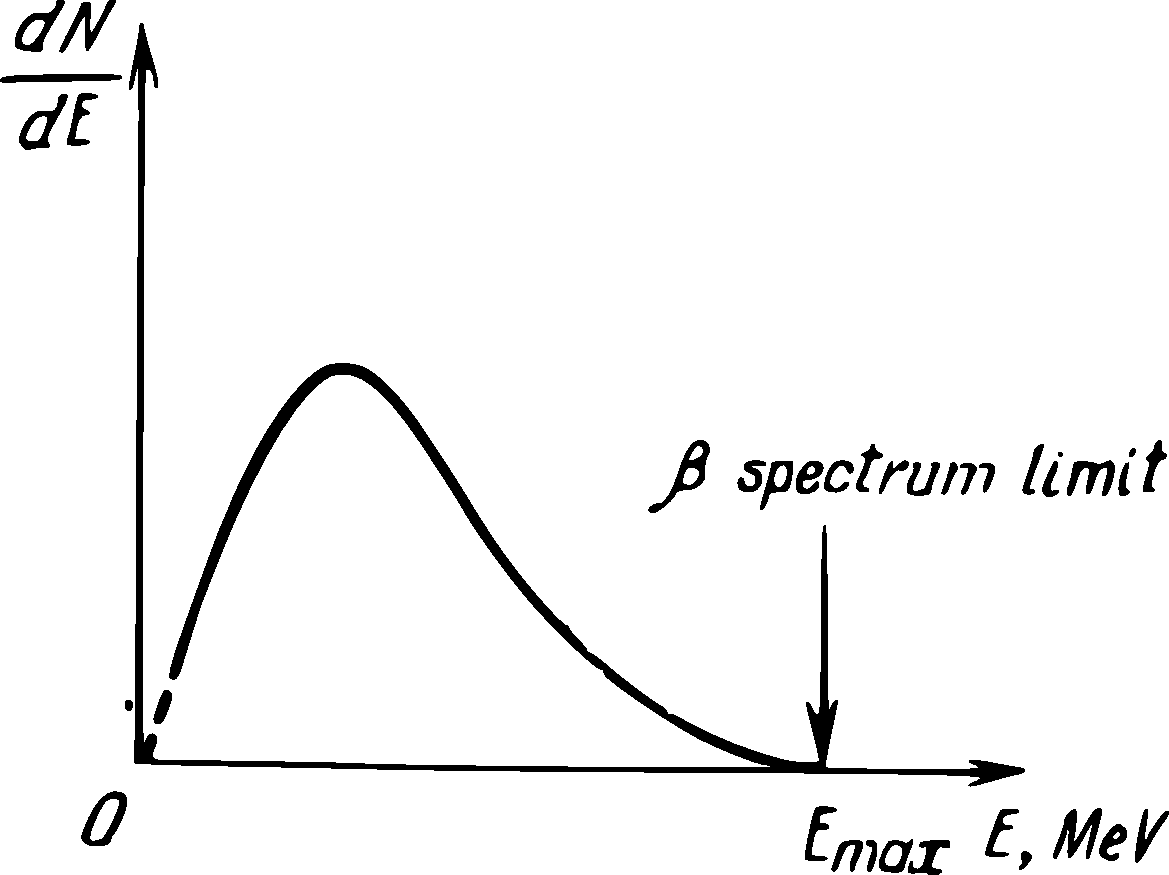
\includegraphics[width=\textwidth]{figs/ch-42/fig-42-02.pdf}
\sidecaption{The energy specture on $\beta^{-}$ decay.\zhcap{$\beta^{-}$ 衰变的能谱。}\label{fig-42-02}}
\end{marginfigure}

\subsection{}\label{42.6.5} The decisive experimental fact in understanding the mechanism of $\beta^{-}$ decay and establishing a suitable theory was an investigation of the energy spectrum of the emitted electrons. This spectrum was found to be continuous, extending to $E = E_{max}$ (\figr{fig-42-02}). The energy $E_{max}$ is called the \redem{upper energy limit} of the $\beta^{-}$ spectrum; it is a characteristic of the source of $\beta^{-}$ radioactive radiation. Electrons with an energy exceeding $E_{max}$ cannot be obtained with the given source.
\zhpar{认识 $\beta^{-}$ 衰变机制并建立适当理论的决定性实验事实，是对所发射电子能谱的研究。该能谱是连续的，延伸至 $E = E_{max}$（见\figr{fig-42-02}）。能量 $E_{max}$ 称为 $\beta^{-}$ 谱的\redem{能量上限}，它是 $\beta^{-}$ 放射源的特征量。用给定的源无法获得能量超过 $E_{max}$ 的电子。}



\subsection{}\label{42.6.6} To reconcile the continuity of the electron energy spectrum with the discrete nature of the energy levels of the nucleus \ssect{42.5.5}, it is necessary to assume that, together with the electron \ce{^{0}_{+1}e}, another particle, the electron antineutrino\sidenote[][-1cm]{Antiparticles are discussed in \ssect{43.5.1}.} $\ce{^{0}_{0}\tilde{\nu}_{e}}$, is emitted from the nucleus. The total energy lost by the nucleus in a beta decay is equal to $E_{max}$, but it is variously distributed between the electron and electron antineutrino.\sidenote{It is evident that $E_{max}$ determines the difference $\Delta E_{ik}$ in the energies of two levels of the nucleus.} In particular, the limit point of the curve in \figr{fig-42-02} means that all the energy of the $\beta^{-}$ decay is carried away by the electron. Zero energy of the electron on the curve would correspond to all the energy being carried away by the antineutrino $\ce{^{0}_{0}\tilde{\nu}_{e}}$.
\zhpar{为使电子能谱的连续性与原子核能级的分立性相协调\ssect{42.5.5}，必须假定：与电子 \ce{^{0}_{+1}e} 一起，还有另一种粒子——电子反中微子 $\ce{^{0}_{0}\tilde{\nu}_{e}}$——从原子核中发射出来。$\beta$ 衰变中原子核损失的总能量等于 $E_{max}$，但该能量在电子与电子反中微子之间有不同的分配。特别地，\figr{fig-42-02}中曲线的端点意味着 $\beta$ 衰变的全部能量都由电子带走。曲线上电子能量为零的点，则对应于全部能量都由反中微子 $\ce{^{0}_{0}\tilde{\nu}_{e}}$ 带走。}
\zhpar{注：反粒子在\ssect{43.5.1}中讨论。}
\zhpar{注：显然，$E_{max}$ 决定了原子核两个能级之差 $\Delta E_{ik}$。}


For the $\beta^{-}$ radioactivity of free neutrons $E_{max} = \SI{782}{\kilo\electronvolt}$, which fully corresponds to that discussed in \ssect{42.6.3}.
\zhpar{对于自由中子的 $\beta^{-}$ 放射性，$E_{max} = \SI{782}{\kilo\electronvolt}$，这与\ssect{42.6.3}中的讨论完全一致。}

\subsection{}\label{42.6.7} Neither the mass number $A$ nor the spin of the nucleus \ssect{42.1.5} changes in a beta decay. The conservation of spin is explained by the fact that the spin of the electron antineutrino is $\hbar/2$ (see  \tabl{tab-43.1}), and the combined spins of this particle
and of the electron, also equal to $\hbar/2$, are equal to zero when the spins of the two particles are oppositely oriented.
\zhpar{$\beta$ 衰变中原子核的质量数 $A$ 与自旋\ssect{42.1.5}均不改变。自旋守恒可解释如下：反电子中微子的自旋为 $\hbar/2$（见\tabl{tab-43.1}），电子的自旋也为 $\hbar/2$，当两粒子的自旋方向相反时，二者的总自旋为零。}

\section{Gamma Rays}
\label{sec-42.7} 
\zhtitle{$\gamma$射线}


 
\subsection{}\label{42.7.1} \redem{Gamma rays} constitute hard electromagnetic radiation whose energy is released in nuclear transitions from excited energy states to the ground or less excited states \ssect{42.5.5}, as well as in nuclear reactions. In the first case, according to the Bohr frequency condition \ssect{39.1.6}, the energy of a photon of gamma rays is equal to the difference in the energies of the
final and initial energy levels of the nucleus:
\zhpar{\redem{$\gamma$ 射线}是硬电磁辐射，其能量在原子核从激发能态跃迁到基态或较低激发态时释放\ssect{42.5.5}，也在核反应中释放。在前一种情形中，根据玻尔频率条件\ssect{39.1.6}，$\gamma$ 光子的能量等于原子核终态与初态能级之差：}
\begin{equation*}%
\hbar \nu_{ik} = E_{i} - E_{k} = \Delta E_{ik},
\end{equation*}
where $\nu_{ik}$ is the frequency of the photon corresponding to the transition of the nucleus from the state with energy $E_{k}$ to the state with energy $E$. The magnitude of $\Delta E_{ik}$ is of the order of \SI{0.1}{\mega\electronvolt} and considerably exceeds the difference of the energies of the electron levels in the atom \ssect{39.1.5}. Gamma rays are extremely short-wave electromagnetic radiation of a wavelength not exceeding \SI{d-2}{\nano\meter}, i.e. \SI{0.1}{\angstrom}. The discrete line spectrum of gamma rays is confirmation of the aforesaid (see \ssect{42.7.4}).
\zhpar{式中 $\nu_{ik}$ 为原子核从能量为 $E_{k}$ 的状态跃迁到能量为 $E$ 的状态时所对应光子的频率。$\Delta E_{ik}$ 的量级约为 \SI{0.1}{\mega\electronvolt}，远大于原子中电子能级之差\ssect{39.1.5}。$\gamma$ 射线是极短波的电磁辐射，波长不超过 \SI{d-2}{\nano\meter}，即 \SI{0.1}{\angstrom}。$\gamma$ 射线的线状谱证实了上述论断（见\ssect{42.7.4}）。}


\subsection{}\label{42.7.2} Gamma radiation is not an independent type of radioactivity \ssect{42.4.2}. It accompanies the processes of $\alpha$ and $\beta$ decays and causes no changes in the charge or mass number of nuclei. It has been established that gamma rays are emitted by a daughter nucleus \ssect{42.4.3} which turns out to be excited at the instant it is formed \ssect{42.7.4}. The excited nucleus loses its energy during a time ranging from \qtyrange{d-13}{d-14}{\second}, which is considerably less than the lifetime of the excited atom ($\approx \SI{d-8}{\second}$).
\zhpar{$\gamma$ 辐射不是独立的放射性类型\ssect{42.4.2}。它伴随 $\alpha$ 衰变和 $\beta$ 衰变过程发生，并且不改变原子核的电荷数或质量数。已经确定，$\gamma$ 射线是子核\ssect{42.4.3}在形成瞬间处于激发态时所发射的\ssect{42.7.4}。激发原子核失去其能量所需的时间约为 \qtyrange{d-13}{d-14}{\second}，远小于受激原子的寿命（$\approx \SI{d-8}{\second}$）。}


\subsection{}\label{42.7.3} The origin and properties of gamma rays are confirmed by the laws of \redem{internal conversion} of gamma rays, which consists in photoelectric-effect phenomena \ssect{37.1.1} of the electrons of the atom's inner shells as a result of gamma radiation of its nucleus. Electrons formed by such an internal photoelectric effect are said to be \redem{conversion electrons}.
\zhpar{$\gamma$ 射线的起源与性质由\redem{内转换}规律所证实：内转换是原子内壳层电子因原子核的 $\gamma$ 辐射而产生的光电效应\ssect{37.1.1}。由这种内光电效应产生的电子称为\redem{内转换电子}。}

In many cases all the energy of the gamma rays is expended on internal conversion phenomena, and only conversion electrons are observed instead of gamma radiation. The energy $eV_{n}$ of a conversion photoelectron is related to the energy $h\nu$ of a photon of gamma rays by Einstein's photoelectric emission equation \ssect{37.1.4}:
\zhpar{在许多情形下，$\gamma$ 射线的全部能量都消耗于内转换过程，因此观测到的只有内转换电子，而没有 $\gamma$ 辐射。内转换光电子的能量 $eV_{n}$ 与 $\gamma$ 光子能量 $h\nu$ 之间的关系，由爱因斯坦光电发射方程\ssect{37.1.4}给出：}
\begin{equation*}%
eV_{n} = h\nu - \Phi_{n},
\end{equation*}
where $\Phi_{n}$ is the work function of an electron from the $n$-th electron shell of the atom, numerically equal to the energies of electrons located at definite energy levels in the atom \ssect{39.1.5}.
\zhpar{式中 $\Phi_{n}$ 为原子第 $n$ 个电子壳层中电子的逸出功，其数值等于原子中处于确定能级上的电子的能量\ssect{39.1.5}。}

These energies are known from data on characteristic $X$-ray
spectra of atoms \ssect{39.7.9}. A gamma photon of the energy $h\nu$ can remove an electron from any inner shell ($K$, $M$, etc.) of the atom \ssect{39.3.6}. Accordingly, the energies $eV_{n}$ of the conversion electrons are expressed by
\zhpar{这些能量可由原子的特征 $X$ 射线谱数据得知\ssect{39.7.9}。能量为 $h\nu$ 的 $\gamma$ 光子可以从原子的任一内壳层（$K$、$M$ 等）打出电子\ssect{39.3.6}。因此，内转换电子的能量 $eV_{n}$ 由下式表示：}
\begin{align*}%
eV_{L} & = h\nu - \Phi_{L},\\
eV_{M} & = h\nu - \Phi_{M},\\
eV_{N} & = h\nu - \Phi_{N}, \text{ etc.}
\end{align*}
where $\Phi_{L}$, $\Phi_{M}$, $\Phi_{N}$, etc. are the $X$-ray energy levels of the atom.
\zhpar{式中 $\Phi_{L}$、$\Phi_{M}$、$\Phi_{N}$ 等为原子的 $X$ 射线能级。}


\subsection{}\label{42.7.4} The result of internal conversion \ssect{42.7.3} is the loss of electrons from the inner shells of the atom and, consequently, the provision of conditions for producing the $X$-ray characteristic spectrum \ssect{39.7.9}. Internal conversion is accompanied by the emission of characteristic $X$-rays. A measurement of the energy of the conversed electrons and the data on the quantities $\Phi_{L}$, $\Phi_{M}$, $\Phi_{N}$, etc. \ssect{42.7.3} enabled it to be shown that the nucleus can emit a definite series of monochromatic gamma rays, i.e. that gamma rays have a line spectrum. Besides, these data showed that gamma rays are emitted by a daughter nucleus rather than a parent one.
\zhpar{内转换的结果是原子内壳层电子的丢失，从而为产生 $X$ 射线特征谱创造了条件\ssect{39.7.9}。内转换伴随着特征 $X$ 射线的发射。通过测量内转换电子的能量，并结合 $\Phi_{L}$、$\Phi_{M}$、$\Phi_{N}$ 等数据\ssect{42.7.3}，可以证明原子核能够发射一系列确定的单色 $\gamma$ 射线，即 $\gamma$ 射线具有线状谱。此外，这些数据还表明 $\gamma$ 射线是由子核而非母核发射的。}

\subsection{}\label{42.7.5} Gamma rays have a very strong effect on matter, in particular, on biological substances. The effect of gamma rays and other kinds of ionizing radiation is evaluated by the absorbed \redem{radiation dose} $D$, the ratio of the energy of radiation to the mass of the irradiated matter. The unit of the dose is \si{\joule\per\kilo\gram}, which is the dose of absorbed radiation at which a mass of \SI{1}{\kilo\gram} of irradiated matter receives \SI{1}{\joule} of energy of ionizing radiation.\sidenote{Owing to the specific nature of information on the biological effect of gamma rays, the pertinent units of physical quantities are given here instead of in the Appendix.} This unit is called the \redem{gray} (\si{\gray}). Also used is the off-system unit called the rad: $1~\text{rad} = \SI{d-2}{\gray}$.
\zhpar{$\gamma$ 射线对物质，特别是对生物物质，有很强的作用。$\gamma$ 射线及其他电离辐射的作用，用被吸收的\redem{辐射剂量} $D$ 来评价，它是辐射能量与受辐照物质质量之比。剂量的单位为 \si{\joule\per\kilo\gram}，即质量为 \SI{1}{\kilo\gram} 的受辐照物质接收到 \SI{1}{\joule} 电离辐射能量时的剂量。该单位称为\redem{戈瑞}（\si{\gray}）。另有一种非国际单位制单位称为拉德：$1~\text{rad} = \SI{d-2}{\gray}$。}
\zhpar{注：由于 $\gamma$ 射线生物效应相关信息的特殊性，此处给出的是相关物理量的单位，而不是附录中的单位。}

The \redem{dose rate $N$ of radiation} is the absorbed dose $D$ referred to unit time. Thus 
\zhpar{辐射的\redem{剂量率} $N$ 是单位时间内的吸收剂量 $D$。即}
\begin{equation*}
N = \frac{D}{t}.
\end{equation*} 
The unit of dose rate is a watt per kilogram: \si{\watt\per\kilo\gram} = \si{\gray\per\second}.
\zhpar{剂量率的单位为瓦特每千克：\si{\watt\per\kilo\gram} = \si{\gray\per\second}。}


\subsection{}\label{42.7.6} The energy characteristic of radiation, evaluated on the basis of the ionization of dry atmospheric air, is the \redem{exposure dose} $D_{e}$. It is measured in coulombs per kilogram (\si{\coulomb\per\kilo\gram}). One coulomb per kilogram of exposure dose of $X$ or gamma radiation is the amount at which the sum of the electric charges of ions of the same sign, produced by the electrons released by irradiated air of \SI{1}{\kilo\gram} mass, fully utilizing the ionizing capacity, is equal to one coulomb. An off-system unit of exposure dose is the \redem{roentgen} R, with $1~\text{R} = \SI{2.58d-4}{\coulomb\per\kilo\gram}$.
\zhpar{根据干燥大气空气的电离作用所评价的辐射能量特征量，称为\redem{照射剂量} $D_{e}$，其单位为库仑每千克（\si{\coulomb\per\kilo\gram}）。X 射线或 $\gamma$ 射线的照射剂量为每千克 1 库仑，是指：在充分利用其电离能力的条件下，质量为 \SI{1}{\kilo\gram} 的受辐照空气所释放的电子所产生的同号离子电荷之和等于 1 库仑。照射剂量的非国际单位为\redem{伦琴}（R），$1~\text{R} = \SI{2.58d-4}{\coulomb\per\kilo\gram}$。}

With an exposure dose equal to 1~R, a total charge of ions of the same charge equal to $(1/3) \times \SI{d-9}{\coulomb}$ is obtained in \SI{d-6}{\meter\cubed} of dry air at standard atmospheric pressure. 
\zhpar{照射剂量为 1 R 时，在标准大气压下，\SI{d-6}{\meter\cubed} 干燥空气中可获得同号离子的总电荷量为 $(1/3) \times \SI{d-9}{\coulomb}$。}

The \redem{exposure dose rate} $N_{e}$ is the exposure dose per unit time: $N_{e} = D_{e}/t$, measured in amperes per kilogram (\si{\ampere\per\kilo\gram}). One unit of exposure dose rate is the electromagnetic radiation at which the exposure dose increases by one coulomb per kilogram in one second. The off-system units of the exposure dose rate 
are: 
\zhpar{\redem{照射剂量率} $N_{e}$ 是单位时间内的照射剂量：$N_{e} = D_{e}/t$，以安培每千克（\si{\ampere\per\kilo\gram}）为单位。照射剂量率的一个单位是这样的电磁辐射：它使照射剂量每秒增加 1 库仑每千克。照射剂量率的非国际单位为：}
\begin{align*}%
1~\text{R/s} & = \SI{2.58d-4}{\ampere\per\kilo\gram},\\
1~\text{R/min} & = \SI{4.30d-6}{\ampere\per\kilo\gram},\\
1~\text{R/h} & = \SI{7.17d-8}{\ampere\per\kilo\gram}.
\end{align*}

\subsection{}\label{42.7.7} A radiation dose can also be evaluated on the basis of its biological effect. The unit applied for this purpose is called the \redem{roentgen equivalent man} (rem). This is the absorbed energy of radiation that produces the same biological effect as that produced by one roentgen. Thus 
\zhpar{辐射剂量也可以根据其生物效应来评价。为此目的所用的单位称为\redem{雷姆}（伦琴当量人，rem）。它是指产生与一个伦琴所产生的生物效应相同的辐射吸收能量。即}
\begin{equation*}%
1~\text{rem} = \SI{d-2}{\joule\per\kilo\gram}.
\end{equation*}
The safe dose rate for humans is considered to be one about
250 times that produced by the background of space and by radioactive radiation from the earth's interior.
\zhpar{人体的安全剂量率被认为约为宇宙空间本底以及地球内部放射性辐射所产生剂量率的 250 倍。}

\section{M\"ossbauer Effect}
\label{sec-42.8} 
\zhtitle{穆斯堡尔效应}


\subsection{}\label{42.8.1} All excited energy levels of the nucleus have energy values determined to an accuracy of $\Delta E$, which is determined from the indeterminacy relation (38.6.6). Thus
\zhpar{原子核所有激发能级的能量值都有确定的精度 $\Delta E$，它由不确定关系（38.6.6）确定。于是有}
\begin{equation*}%
\Delta E = \frac{\hbar}{\Delta t},
\end{equation*}
where $\Delta t$ is the lifetime of the nucleus in the excited state. Only for the ground state of a stable nucleus is $\Delta t = \infty$ and $\Delta E = 0$, i.e. the energy value of the nucleus is exactly equal to $E$.\sidenote{This is equally true for the energy levels of electrons in atoms.} For example, a nucleus of iridium \ce{^{191}_{77}Ir} goes over from the excited state with the energy $E = \SI{129}{\keV}$ to the ground state, emitting a gamma photon, during the time $\Delta t$, which can be taken equal to the half-life \ssect{42.4.5} $T  = \SI{d-10}{\second}$. The
energy indeterminacy $\Delta E$ is found to equal $\Delta E \approx  \SI{5d-6}{\eV}$.
\zhpar{式中 $\Delta t$ 为原子核处于激发态的寿命。只有稳定原子核的基态满足 $\Delta t = \infty$ 和 $\Delta E = 0$，即原子核的能量值恰好等于 $E$。例如，铱核 \ce{^{191}_{77}Ir} 从能量为 $E = \SI{129}{\keV}$ 的激发态跃迁到基态并发射一个 $\gamma$ 光子，所用时间 $\Delta t$ 可取为半衰期\ssect{42.4.5} $T  = \SI{d-10}{\second}$。能量的不确定量 $\Delta E$ 约为 $\Delta E \approx  \SI{5d-6}{\eV}$。}
\zhpar{注：对于原子中电子的能级，这一点同样成立。}

The finite lifetime of the excited energy states of the nucleus leads to a lack of monochromaticity of the gamma radiation that accompanied the transition of the nucleus from the excited to the ground state. This lack of monochromaticity is called the \redem{natural linewidth} of gamma radiation, and the indeterminacy $\Delta E$ of the energy of an excited state is called the \redem{natural width $\Gamma$ of the energy level of the nucleus}.\sidenote{This definition also holds for transitions of atoms from an excited to the ground state. But here the lack of monochromaticity is called the \redem{natural spectral linewidth}, and the indeterminacy is the \redem{natural width of energy levels of electrons} in the atom.}
\zhpar{原子核激发能态的寿命有限，导致原子核从激发态跃迁到基态时所发出的 $\gamma$ 辐射不具有完全的单色性。这种单色性的不足称为 $\gamma$ 辐射的\redem{自然线宽}，而激发态能量的不确定量 $\Delta E$ 称为原子核能级的\redem{自然宽度 $\Gamma$}。}
\zhpar{注：这一定义同样适用于原子从激发态跃迁到基态的情形。但此时单色性的不足称为\redem{自然谱线宽度}，而其不确定量则是原子中电子能级的\redem{自然宽度}。}

\subsection{}\label{42.8.2}  \redem{Resonance absorption} of gamma rays by nuclei implies the absorption by the nuclei of gamma photons of such frequency $\nu$ that the energy $h\nu$ of a photon is equal to the difference in the energies of one of the excited states and the ground state of the nucleus. The name means that the line of the gamma photon, emitted in the transition of the nucleus from an excited state to its ground state, has the same frequency $\nu$.
\zhpar{$\gamma$ 射线的\redem{共振吸收}是指原子核吸收频率为 $\nu$ 的 $\gamma$ 光子，其能量 $h\nu$ 等于原子核某一激发态与基态的能量差。这一名称的含义是：原子核由激发态跃迁到基态时所发出的 $\gamma$ 光子谱线，具有相同的频率 $\nu$。}

When gamma photons are emitted or absorbed by a nucleus, the
 \redem{recoil of the nucleus} is taken into account. In a transition of a nucleus from an excited state with the energy E to the ground state (of an energy taken equal to zero), the gamma photon acquires the energy £ph equal to
\zhpar{原子核发射或吸收 $\gamma$ 光子时，应考虑\redem{原子核的反冲}。在原子核从能量为 $E$ 的激发态跃迁到能量取为零的基态时，$\gamma$ 光子所获得的能量 $E_{ph}$ 为}
\begin{equation*}%
h \nu_{em} = E_{ph} = E - E_{N}  < E,
\end{equation*} 
where $E_{N}$ is the nuclear recoil energy.
\zhpar{式中 $E_{N}$ 为原子核的反冲能量。}

In exciting the nucleus and its transition from the ground state to the state with the energy $E$, the gamma photon should have the energy $E_{ph}'$, equal to $h\nu_{abs} = E_{ph}' = E + E_{N} > E$.
\zhpar{使原子核从基态激发到能量为 $E$ 的状态时，$\gamma$ 光子应具有能量 $E_{ph}'$，其值等于 $h\nu_{abs} = E_{ph}' = E + E_{N} > E$。}

The frequencies at the maxima of the emission lines $(\nu_{em})$ and absorption lines $(\nu_{abs})$ are shifted with respect to one another by the amount
\zhpar{发射谱线（$\nu_{em}$）与吸收谱线（$\nu_{abs}$）极大值处的频率相差如下量：}
\begin{equation*}%
\nu_{abs} - \nu_{em} = \Delta \text{ such that } h \Delta \nu = 2 E_{N}.
\end{equation*} 
The energy $E_{N}$ of nuclear recoil can be determined from the momentum $\vb{p}_{ph}$ of the photon \ssect{37.2.2}, which, in the processes of emitting and absorbing a gamma photon, should equal the momentum of the nucleus $(\vb{p}_{ph} - \vb{p}_{N})$:
\zhpar{反冲能量 $E_{N}$ 可由光子的动量 $\vb{p}_{ph}$ 求得\ssect{37.2.2}。在发射与吸收 $\gamma$ 光子的过程中，光子动量应等于原子核的动量 $(\vb{p}_{ph} - \vb{p}_{N})$，于是有}
\begin{equation*}%
E_{N} = \frac{p^{2}_{N}}{2M_{N}} =\frac{p^{2}_{ph}}{2M_{N}} = \left( \frac{h \nu}{c}\right)^{2} \frac{1}{2M_{N}},
\end{equation*}
where $M_{N}$ is the mass of the nucleus. For the nucleus \ce{^{191}_{77}Ir}, with the energy $E = \SI{129}{\keV}$ of its excited state, calculations yield $E_{N} = \SI{0.05}{\eV}$ and a shift $\Delta \nu = 2E_{N}/h$ of the maxima of
emission and absorption lines. At this, $h \Delta \nu = \SI{0.1}{\eV}$, which considerably exceeds the natural width of level $\Gamma$ \ssect{42.8.1}.
\zhpar{式中 $M_{N}$ 为原子核的质量。对于激发态能量为 $E = \SI{129}{\keV}$ 的铱核 \ce{^{191}_{77}Ir}，计算得 $E_{N} = \SI{0.05}{\eV}$，发射与吸收谱线极大值的频移为 $\Delta \nu = 2E_{N}/h$。此时 $h \Delta \nu = \SI{0.1}{\eV}$，远大于能级的自然宽度 $\Gamma$\ssect{42.8.1}。}

\subsection{}\label{42.8.3} A drastic reduction in the energy of nuclear recoil in absorbing and emitting gamma rays is evident when these processes are observed in nuclei in the crystal lattice, i.e. in the bound state. Under these conditions, the momentum and energy are imparted to the crystal lattice as a whole, rather than to the single nucleus that emits (or absorbs) a gamma photon. The mass of the crystal is substantially greater than that of a nucleus,
and the loss of energy E- in emission or absorption of gamma
rays becomes extremely small. In this case, resonance absorption and emission of a gamma photon of a strictly dehnite frequency $\nu$ is observed and the linewidth is comparable to the natural width \ssect{42.8.1}. The phenomenon of resonance absorption (or emission) of gamma rays without recoil is called the \redem{M\"ossbauer effect}.
\zhpar{当原子核处于晶格中，即处于束缚态时，吸收与发射 $\gamma$ 光子所引起的反冲能量会大幅减小。在这种条件下，动量和能量传递给整个晶体，而不是仅传递给发射（或吸收）$\gamma$ 光子的单个原子核。晶体的质量远大于原子核的质量，因此在发射或吸收 $\gamma$ 射线时的能量损失变得极小。此时可以观测到严格确定频率 $\nu$ 的 $\gamma$ 光子的共振吸收与发射，且谱线宽度与自然宽度相当\ssect{42.8.1}。这种无反冲的 $\gamma$ 射线共振吸收（或发射）现象称为\redem{穆斯堡尔效应}。}

\subsection{}\label{42.8.4} The M\"ossbauer effect is made use of in \redem{nuclear spectroscopy} to make precise measurements of the energy levels of atomic nuclei. In the gamma transition in \ce{^{57}Fe} nuclei, for instance,
with the energy of the transition $E = \SI{14.1}{\keV}$, the change in the energy of the level is determined with an accuracy to $\Gamma/E = \num{3d-13}$. For the gamma transition in \ce{^{67}Zn} with the energy of the transition $E = \SI{93}{\keV}$, the quantity $\Gamma/E$ was found to
equal \num{5d-16}.
\zhpar{穆斯堡尔效应被用于\redem{核谱学}，以精确测量原子核的能级。例如，对于 \ce{^{57}Fe} 核的 $\gamma$ 跃迁，其跃迁能量为 $E = \SI{14.1}{\keV}$，能级能量的变化可精确到 $\Gamma/E = \num{3d-13}$。对于 \ce{^{67}Zn} 的 $\gamma$ 跃迁，其跃迁能量为 $E = \SI{93}{\keV}$，测得的 $\Gamma/E$ 为 \num{5d-16}。}

The M\"ossbauer effect has been used to check the conclusion on shift of spectral line frequencies in a gravitational field \ssect{6.2.1}. As a photon travels in a gravitational field its energy is changed by the amount $\Delta E = -m (\varphi_{2} - \varphi_{1})$, where $m = h\nu/c^{2}$ is the mass of the photon \ssect{37.2.1}, and $\varphi_{1}$ and $\varphi_{2}$ are the potentials of the gravitational held at points $\mathit{1}$ and $\mathit{2}$ \ssect{6.2.4}. The minus sign indicates that the increase in the energy of a photon in a gravitational held is at the expense of its own energy $E = h\nu$:
\zhpar{穆斯堡尔效应已被用于检验光谱线频率在引力场中移动的结论\ssect{6.2.1}。光子在引力场中运动时，其能量改变量为 $\Delta E = -m (\varphi_{2} - \varphi_{1})$，式中 $m = h\nu/c^{2}$ 为光子的质量\ssect{37.2.1}，$\varphi_{1}$ 和 $\varphi_{2}$ 分别为引力场中 $\mathit{1}$、$\mathit{2}$ 两点的引力势\ssect{6.2.4}。负号表示光子在引力场中能量的增加是以其自身能量 $E = h\nu$ 为代价的：}
\begin{equation*}%
h \Delta \nu = -m \Delta \varphi.
\end{equation*}
The relative change in frequency of a photon as it passes through a gravitational potential difference Acp is
\zhpar{光子通过引力势差 $\Delta \varphi$ 时，其频率的相对变化为}
\begin{equation*}%
\frac{\Delta \nu}{ \nu} = \frac{\Delta \varphi}{c^{2}},
\end{equation*}
Here $\Delta \varphi > 0$ because the potential of zero gravity of the sun increases with the distance from the sun. At the earth's surface it is greater than at that of the sun. Consequently, $\Delta \nu / \nu < 0$ and all frequencies of spectral lines of the sun and stars, recorded on the earth, are shifted toward the red end of the spectrum. This effect is called the \redem{gravitational red shift}. 
\zhpar{这里 $\Delta \varphi > 0$，因为太阳的零引力势随离开太阳的距离增大而增大；地球表面处的该值大于太阳表面处的值。因此 $\Delta \nu / \nu < 0$，地球上所测得的太阳与恒星各谱线频率都向光谱的红端移动。这种效应称为\redem{引力红移}。}

The M\"ossbauer effect enabled the gravitational frequency 
shift of the gamma photon to be observed in its motion in the earth's gravitational field. In vertical motion from the floor to the ceiling of the laboratory to a height of about \SI{10}{\meter}, the relative change in frequency is
\zhpar{穆斯堡尔效应使人们能够观测 $\gamma$ 光子在地球引力场中运动时的引力频移。在实验室中，光子从地板竖直上升到天花板，高度约 \SI{10}{\meter}，此时频率的相对变化为}
\begin{equation*}%
\abs{\frac{\Delta \nu}{ \nu}} = \frac{\Delta \varphi}{c^{2}} = \frac{g \Delta h}{c^{2}} \approx \num{d-15}, 
\end{equation*}
where $g$ is the acceleration due to gravity \ssect{7.3.3}. To record this frequency shift it is necessary to provide for resonance absorption of gamma photons in such manner that the source and detector of the gamma rays have a relative linewidth equal to or less than \num{d-15}. Then there will be no absorption if the frequency of the gamma photon incident on the nucleus differs from the frequency of the photon that the nucleus can absorb by the amount $\Delta \nu = \num{d-15} \nu$.
\zhpar{式中 $g$ 为重力加速度\ssect{7.3.3}。为记录这一频移，必须使 $\gamma$ 光子的共振吸收满足：$\gamma$ 射线的源与探测器的相对线宽等于或小于 $\num{d-15}$。这样，若入射到原子核上的光子频率与该核能够吸收的光子频率相差 $\Delta \nu = \num{d-15} \nu$，则不会发生吸收。}

This experiment was conducted with two identical crystal
sources of gamma rays, one of which could be placed at a height of \SI{20}{\meter} above the other. When the detector of gamma photons was at the same height as the source of gamma photons, resonance absorption occurred. As the detector was raised \SI{20}{\meter} the absorption ceased owing to the gravitational shift in frequency.
\zhpar{该实验使用两个相同的晶体 $\gamma$ 源进行，其中一个可以放置在另一个上方 \SI{20}{\meter} 处。当 $\gamma$ 光子探测器与 $\gamma$ 光子源处于同一高度时，发生共振吸收。当探测器升高 \SI{20}{\meter} 后，由于引力引起的频率移动，吸收便消失了。}

The Doppler effect \ssect{30.6.1} was employed to restore absorption. At a definite velocity at which the detector and source approach each other, the Doppler increase in frequency exactly compensated for its gravitational reduction, and resonance absorption was restored. This experiment was a confirmation under laboratory conditions of the gravitational red shift.
\zhpar{利用多普勒效应\ssect{30.6.1}使吸收得以恢复。当探测器与源以一定速度相互接近时，多普勒引起的频率增加恰好补偿了引力引起的频率降低，共振吸收随之恢复。该实验在实验室条件下证实了引力红移。}

\section{Nuclear Reactions}
\label{sec-42.9} 
\zhtitle{核反应}


\subsection{}\label{42.9.1} \redem{Nuclear reactions} are transformations of atomic nuclei brought about by their interactions with one another or with elementary particles \ssect{43.1.1}. As a rule, nuclear reactions involve
two nuclei and two particles. One pair, a nucleus and a
particle, is said to be the \redem{initial}, and the other, the \redem{final} pair.
\zhpar{\redem{核反应}是原子核之间，或原子核与基本粒子\ssect{43.1.1}相互作用而引起的原子核转变。通常，核反应涉及两个原子核和两个粒子。其中一对（一个原子核和一个粒子）称为\redem{初态}，另一对称为\redem{终态}。}

Nuclear reactions are represented in one of the following ways:
\zhpar{核反应可用以下方式之一表示：}
\begin{equation*}%
A + a \to B + b \qor A \,(a,\, b)\, B,
\end{equation*}
where $A$ and $B$ are the initial and final nuclei, and $a$ and $b$ are the initial and final particles in the reaction. In many cases a nuclear reaction can proceed in more than one way, the preceding reaction being $A + a \to C + c$, i.e. $A\, (a,\, c) \,C$, or some other version. The possible ways in which a nuclear reaction may proceed are called its \redem{channels}. The initial phase of a reaction is called its \redem{entrance channel}.
\zhpar{式中 $A$ 和 $B$ 分别为初始和最终的原子核，$a$ 和 $b$ 分别为反应中的初始和最终粒子。在许多情形中，核反应可以以不止一种方式进行，例如核反应也可以是 $A + a \to C + c$，即 $A\, (a,\, c) \,C$，或其他形式。核反应可能进行的各种方式称为其\redem{反应道}。反应的初始阶段称为其\redem{入射道}。}

\subsection{}\label{42.9.2} A nuclear reaction is characterized by its energy $Q$ (called the \redem{nuclear reaction energy}), which is equal to the difference
between the energies of the final and initial pairs in the reaction \ssect{42.9.1}. When $Q < 0$, the reaction proceeds with the absorption of energy and is said to be \redem{endothermic} (or \redem{endoenergic}) when $Q > 0$, the reaction proceeds with the release of energy and is said to be \redem{exothermic} (or \redem{exoergic}). An endothermic nuclear reaction is found to be feasible at a certain minimum (threshold) kinetic energy $E_{th}$ of the nuclei or particles causing the reaction:
\zhpar{核反应的特征量是其\redem{核反应能} $Q$，它等于反应中终态两粒子对的能量与初态两粒子对的能量之差\ssect{42.9.1}。当 $Q < 0$ 时，反应吸收能量，称为\redem{吸能反应}（或\redem{吸能}）；当 $Q > 0$ 时，反应释放能量，称为\redem{放能反应}（或\redem{放能}）。吸能核反应只有在引起反应的原子核或粒子具有一定的最低（阈）动能 $E_{th}$ 时才能发生：}
\begin{equation*}%
E_{th} = \frac{M_{A}+ M_{a}}{M_{A}}Q,
\end{equation*}
where $M_{A}$ is the mass of the stationary (target) nucleus, and $M_{a}$ is the mass of the particle (or nucleus) bombarding the target nucleus. 
\zhpar{式中 $M_{A}$ 为静止（靶）原子核的质量，$M_{a}$ 为轰击靶核的粒子（或原子核）的质量。}

Nuclear reactions comply with the laws of conservation of energy, momentum, electrical charge and mass number. If the kinetic energy of the particles entering a reaction is sufficient for the creation of a nucleon-antinucleon pair \ssect{43.5.6}, the mass number may change. Besides, nuclear physics has certain conservation laws not found in other branches of physics (see \ssect{43.4.1} through \ssect{43.4.4}).
\zhpar{核反应遵守能量守恒、动量守恒、电荷守恒和质量数守恒定律。若入射粒子的动能足以产生一个核子-反核子对\ssect{43.5.6}，则质量数可能发生改变。此外，核物理还具有一些其他物理分支中所没有的守恒定律（参见\ssect{43.4.1}至\ssect{43.4.4}）。}

\subsection{}\label{42.9.3} The efficiency of a nuclear reaction is determined by the magnitude of the effective cross section a of the given reaction (reaction cross section). Quantity $\sigma$ has the dimension of area and characterizes the ``yield'' of the reaction per particle
irradiating the nucleus. Thus
\zhpar{核反应的效率取决于该反应的有效截面 $\sigma$（反应截面）的大小。量 $\sigma$ 具有面积的量纲，它表征了每个入射到原子核上的粒子所产生的反应“产额”。即}
\begin{equation*}%
\sigma = \frac{\dd n_{0}}{n_{0}N_{0} \dd x} 
\end{equation*}
It is assumed in this definition that a plane-parallel stream, containing $n_{0}$ particles is incident in unit time on unit area of the cross section of a substance containing $N_{0}$ nuclei in unit volume; $\dd n_{0}$ is the number of the particles that undergo the nuclear reaction in a layer of the thickness $\dd x$.
\zhpar{在此定义中假定：单位时间内，含有 $n_{0}$ 个粒子的平行平面粒子流垂直入射到单位截面积的物质上，该物质单位体积内含有 $N_{0}$ 个原子核；$\dd n_{0}$ 为在厚度为 $\dd x$ 的薄层中发生核反应的粒子数。}

\subsection{}\label{42.9.4} Depending upon the nature of the interaction of particle a with the target $A$, distinction is made between \redem{direct interaction}, in which nuclear reactions proceed in a single stage according to some process \ssect{42.9.1} and nuclear reactions that proceed
in two stages with the formation of a \redem{compound nucleus}.
\zhpar{根据入射粒子 $a$ 与靶核 $A$ 相互作用的性质，核反应可以分为两类：一类是\redem{直接相互作用}，即核反应在单一阶段内按某种过程完成\ssect{42.9.1}；另一类是分两个阶段进行、并形成\redem{复合核}的核反应。}

In the first stage the incident particle is captured by the target nucleus and the particle's energy is not imparted to any particular nucleon, but is shared equally by all the particles of the compound nucleus. Thus none of the particles gains sufficient energy to be ejected from the nucleus.\sidenote{The ``missile'' captured by the nucleus, for instance, an alpha particle or deuteron, can consist of several particles.} The compound nucleus is dealt with as an excited statistical system of particles, having random motions similar to those of particles in a drop of liquid.
Such rapid redistribution of energy between the particles of the nucleus is possible only upon frequent collisions of the particles, this being typical for the redistribution of energy between the particles in a drop of liquid. As the result of chance deviations from uniform distributions of the excitation energy amongst the particles of the compound nucleus, sufficient energy is concentrated on one of them to be ejected from the nucleus. This second stage of the nuclear reaction occurs after a lapse of time (\numrange{d7}{d8}) $\tau_{N}$ following the first stage, where $\tau_{N}$  is the characteristic nuclear time \ssect{43.2.6}.
\zhpar{在第一阶段，入射粒子被靶核俘获，粒子的能量并不转移给某一特定的核子，而是由复合核中的所有粒子均分，因此没有任何一个粒子获得足够的能量逸出原子核。复合核被看作一个激发的统计系统，其中粒子作类似于液滴中粒子的无规运动。这种能量在原子核中粒子间的快速重新分布，只有在粒子频繁碰撞的条件下才可能实现，这与液滴中粒子间能量的重新分布相似。由于激发能在复合核各粒子间的分布偶然地偏离均匀状态，足够的能量会集中到其中某一粒子上，使其逸出原子核。核反应的第二阶段在第一阶段之后经过时间 $(\numrange{d7}{d8}) \tau_{N}$ 发生，其中 $\tau_{N}$ 为原子核的特征时间\ssect{43.2.6}。}
\zhpar{注：被原子核俘获的“弹丸”，例如 $\alpha$ 粒子或氘核，可以由若干个粒子组成。}

The sequence of a nuclear reaction proceeding with the formation of a compound nucleus is as follows:
\zhpar{经复合核形成的核反应过程如下：}
%\begin{equation*}%
%\nuc{X}{A_{1}}{Z_{1}} + \mathrm{a} \to \nuc{Y}{A_{2}}{Z_{2}} \to \nuc{C}{A_{3}}{Z_{3}} + \mathrm{b},
%\end{equation*}
\begin{equation*}%
^{\mathrm{A}_{1}}_{\mathrm{Z}_{1}}\mathrm{X} + \mathrm{a} \to ^{\mathrm{A}_{2}}_{\mathrm{Z}_{2}}\mathrm{Y} \to ^{\mathrm{A}_{3}}_{\mathrm{Z}_{3}}\mathrm{C} + \mathrm{b},
\end{equation*}
where $^{\mathrm{A}_{1}}_{\mathrm{Z}_{1}}\mathrm{X}$ is the initial target nucleus, a is the incident particle, $^{\mathrm{A}_{2}}_{\mathrm{Z}_{2}}\mathrm{Y}$ is the compound nucleus, is the product nucleus $^{\mathrm{A}_{3}}_{\mathrm{Z}_{3}}\mathrm{C}$ and b is the particle ejected from the nucleus as a result of the reaction.
\zhpar{式中 $^{\mathrm{A}_{1}}_{\mathrm{Z}_{1}}\mathrm{X}$ 为初始靶核，a 为入射粒子，$^{\mathrm{A}_{2}}_{\mathrm{Z}_{2}}\mathrm{Y}$ 为复合核，$^{\mathrm{A}_{3}}_{\mathrm{Z}_{3}}\mathrm{C}$ 为产物核，b 为反应中从原子核发射出的粒子。}

If $\mathrm{a} = \mathrm{b}$, particles are being scattered by the nucleus (scattering is elastic or inelastic according to whether the energy of the particles is the same or different before and after scattering). If $\mathrm{b} \neq \mathrm{a}$, a nuclear reaction is proceeding in the true sense of the term.
\zhpar{若 $\mathrm{a} = \mathrm{b}$，则粒子被原子核散射（根据散射前后粒子能量相同或不同，分为弹性散射或非弹性散射）。若 $\mathrm{b} \neq \mathrm{a}$，则发生严格意义上的核反应。}

\subsection{}\label{42.9.5} Nuclear reactions are classified according to various of their features: according to the energy of the particles that initiate them, according to the energy of the particles partici­ pating in them, and according to the nature of the nuclear transformations
that occur in them. Nuclear reactions at low energies
(of the order of \SI{1}{\eV}) proceed mainly with the participation of neutrons. Reactions at medium energies (up to several \si{\MeV}) are induced, in addition to neutrons, by various charged particles (alpha particles, protons, deuterons, nuclei of heavy hydrogen, etc.), as well as gamma photons. Charged particles that cause nuclear reactions may be multiply charged ions of heavy chemical elements, as well as charged particles accelerated in accelerators. Reactions at high energies (hundreds and thousands of \si{\MeV}) lead to the creation of elementary particles (mesons, hyperons, etc.) that are absent in the free state.
\zhpar{核反应可依据多种特征分类：依据引发反应的粒子能量，依据参与反应的粒子能量，以及依据反应中发生的核转变性质。低能（约 \SI{1}{\eV} 量级）核反应主要由中子参与。中能（直至数 \si{\MeV}）核反应除中子外，还由各种带电粒子（$\alpha$ 粒子、质子、氘核、重氢核等）以及 $\gamma$ 光子引发。引起核反应的带电粒子可以是重化学元素的多电荷离子，也可以是加速器加速的带电粒子。高能（数百至数千 \si{\MeV}）核反应会产生自由态中不存在的基本粒子（介子、超子等）。}

\subsection{}\label{42.9.6} The following are examples of nuclear reactions initiated by alpha particles and deuterons \ce{^{2}_{1}D}:
\zhpar{下列是由 $\alpha$ 粒子和氘核 \ce{^{2}_{1}D} 引发的核反应的例子：}
\begin{enumerate}[label = (\alph*)]
\item historically, the first nuclear reaction for the transformation
of nitrogen into oxygen was the following:
\zhpar{历史上，第一个将氮转变为氧的核反应如下：}
%\begin{equation*}%
%\nuc{N}{14}{7} + \nuc{He}{4}{2} \to ( \nuc{F}{18}{9}) \to \nuc{O}{17}{8} + \nuc{p}{1}{1},
%\end{equation*}
\begin{equation*}%
\ce{^{14}_{7}N} + \ce{^{4}_{2}He} \to ( \ce{^{18}_{9}F}) \to \ce{^{17}_{8}O} + \ce{^{1}_{1}p},
\end{equation*}
or in shorter notation:
\zhpar{也可写成较简略的形式：}
\begin{equation*}
\nuc{N}{14}{7} \, (\alpha, \textrm{p}) \, \nuc{O}{17}{8};
\end{equation*}
\item the nuclear reaction in which neutrons were first obtained was:
\zhpar{首次获得中子的核反应为：}
\begin{equation*}%
\nuc{Be}{9}{4} + \nuc{He}{4}{2} \to \nuc{C}{12}{6} + \nuc{n}{1}{0};
\end{equation*}
\item nuclear reactions initiated by deuterons \ce{^{2}_{1}D}, the nuclei of heavy hydrogen (deuterium), can lead to the fusion of heavy nuclei, tritium \ce{^{3}_{1}H}, or the light isotope of helium \ce{^{3}_{2}He}, with the formation of a proton or neutron:
\zhpar{由氘核 \ce{^{2}_{1}D}（重氢核，即氘）引发的核反应，可以导致轻核聚变，生成氚 \ce{^{3}_{1}H} 或轻的氦同位素 \ce{^{3}_{2}He}，并伴随质子或中子的产生：}
\begin{equation*}%
\nuc{D}{2}{1} + \nuc{D}{2}{1} \to \nuc{H}{3}{1} + \nuc{p}{1}{1} \qand \nuc{D}{2}{1} + \nuc{D}{2}{1} \to \nuc{He}{3}{2} + \nuc{n}{1}{0},
\end{equation*}
(see also \sect{42.9.13}).
\zhpar{（亦见\sect{42.9.13}）。}
\end{enumerate}

\subsection{}\label{42.9.7} The action of neutrons \ce{^{1}_{0}n} leads to the formation of artificial radioactive isotopes, such as radiocarbon  \ce{^{14}_{6}C} with a half-life \ssect{42.4.5} exceeding 5000 years:
\zhpar{中子的作用会生成人工放射性同位素，例如半衰期\ssect{42.4.5}超过 5000 年的放射性碳 \ce{^{14}_{6}C}：}
\begin{equation*}%
\nuc{N}{14}{7} + \nuc{n}{1}{0} \to \nuc{C}{14}{6} + \nuc{p}{1}{1}.\tag{$\star$}
\end{equation*}
Subsequent decay proceeds according to the process
\zhpar{其后的衰变按下列过程进行：}
\begin{equation*}%
\nuc{C}{14}{6} \to  \nuc{N}{14}{7} + \nuc{e}{0}{-1} + ^{0}_{0}\tilde{\nu_{e}}.
\end{equation*}
where $\nuc{e}{0}{-1}$ and $^{0}_{0}\tilde{\nu_{e}}$ represent the electron and electron antineutrino. The long half-life of \ce{^{14}_{6}C} is the basis for the radiocarbon (carbon-14) dating technique used in archaeology. By determining the relative amount of undecayed radioactive carbon, which ceased to be accumulated in a living organism when it died, it is possible, according to reaction ($\star$), to establish the time when the organism no longer absorbed the isotope \ce{^{14}_{6}C} from
the atmosphere. This isotope is formed in the atmosphere from nitrogen by the action of cosmic-ray neutrons.
\zhpar{式中 $\nuc{e}{0}{-1}$ 与 $^{0}_{0}\tilde{\nu_{e}}$ 分别表示电子与电子反中微子。\ce{^{14}_{6}C} 的半衰期较长，这是考古学中放射性碳（碳-14）测年技术的基础。通过测定生物体死亡后已不再积累的放射性碳中未衰变部分的相对含量，并依据反应（$\star$），可以确定生物体停止从大气中吸收同位素 \ce{^{14}_{6}C} 的时间。该同位素是由宇宙射线中子作用于大气中的氮而形成的。}

\subsection{}\label{42.9.8} \redem{Slow neutrons} are ones whose de Broglie wavelength \ssect{38.1.4} exceeds the nuclear radius $R$: $\lambda \gg \hbar/mv$ and, accordingly,
$v \ll \hbar/mR$. Their energy does not exceed \SI{100}{\keV}. Neutrons with energies up to \SI{0.5}{\keV}are called \redem{thermal neutrons}. As such neutrons pass through matter they undergo capture, the absorption of the neutrons by the nuclei. If the energy of the neutrons
coincides with that of the compound nucleus \ssect{42.9.4}, \redem{resonance absorption} (resonance capture) of the neutrons occurs. This process is the basis of the technique for obtaining \redem{transuranic chemical elements}. The transuranic element neptunium \ce{^{239}_{93}Np}
is formed upon resonance capture of neutrons by the most abundant isotope of uranium \ce{^{238}_{92}U} according to the reaction
\zhpar{\redem{慢中子}是指其德布罗意波长\ssect{38.1.4}大于原子核半径 $R$ 的中子：$\lambda \gg \hbar/mv$，因而 $v \ll \hbar/mR$。其能量不超过 \SI{100}{\keV}。能量不超过 \SI{0.5}{\keV} 的中子称为\redem{热中子}。中子通过物质时会被原子核俘获（吸收）。若中子能量恰好与复合核的能量相符\ssect{42.9.4}，则发生中子的\redem{共振吸收}（共振俘获）。这一过程是获得\redem{超铀元素}的技术基础。超铀元素镎 \ce{^{239}_{93}Np} 由丰度最大的铀同位素 \ce{^{238}_{92}U} 共振俘获中子后，按下列反应形成：}
\begin{equation*}
\ce{^{238}_{92}U} + \ce{^{1}_{0}n} \to \ce{^{239}_{92}U} 
\xrightarrow[\text{23 min}]{\beta^{-}}  
\ce{^{239}_{93}Np},
\end{equation*}
where the half-life of radioactive isotope  \ce{^{239}_{92}U} is indicated, which is transformed into \ce{^{239}_{93}Np}. Next, the nucleus of isotope
\ce{^{239}_{93}Np} is transformed into plutonium \ce{^{239}_{94}Pu}:
\zhpar{式中 \ce{^{239}_{92}U} 为放射性同位素（其半衰期已标注于箭头上），它转变为 \ce{^{239}_{93}Np}。接着，同位素 \ce{^{239}_{93}Np} 的原子核转变为钚 \ce{^{239}_{94}Pu}：}
\begin{equation*}
\ce{^{239}_{93}Np} 
\xrightarrow[\text{2.3 days}]{\beta^{-}}  
\ce{^{239}_{94}Pu}.
\end{equation*}
Owing to its efficient fission by the action of thermal neutrons \ssect{42.9.10}, plutonium plays a prominent role in the production of nuclear energy. Plutonium \ce{^{239}_{94}Pu} is radioactive by alpha particle emission and has a huge half-life (24,000 years). It is transformed into the stable isotope of uranium \ce{^{235}_{92}U} according to the
reaction:
\zhpar{由于钚 \ce{^{239}_{94}Pu} 能通过热中子的作用有效地发生裂变\ssect{42.9.10}，它在核能生产中起着重要作用。钚-239 以发射 $\alpha$ 粒子的方式进行放射性衰变，其半衰期极长（24000 年）。它按下列反应转变为稳定的铀同位素 \ce{^{235}_{92}U}：}
\begin{equation*}
\ce{^{239}_{94}Pu}
\xrightarrow[\text{\num{2.4d4} years}]{\alpha} \ce{^{235}_{92}U}.
\end{equation*}

\subsection{}\label{42.9.9} Nuclear reactions using accelerated nuclei of chemical elements enabled advancement in Mendeleev's table up to the (dement with the number $Z = 107$. The element with $Z = 105$ was named nilsbohrium (Ns). Upon bombarding the isotope \ce{^{242}_{94}Pu} with nuclei of neon \ce{^{22}_{10}Ne} a chemical element with $Z = 104$
(kurchatovium \ce{^{260}_{104}Ku}) is obtained. After capture of the nucleus \ce{^{22}_{10}Ne} by plutonium, the compound nucleus of kurchatovium \ce{^{264}_{104}Ku} is formed. Then, in one out of ten thousand million compound
nuclei, the nucleus of the element \ce{^{260}_{104}Ku} was produced after emitting four neutrons. Thus
\zhpar{利用加速的原子核进行核反应，使门捷列夫周期表扩展到原子序数 $Z = 107$ 的元素。原子序数 $Z = 105$ 的元素被命名为 nilsbohrium（Ns）。用氖核 \ce{^{22}_{10}Ne} 轰击同位素 \ce{^{242}_{94}Pu}，可获得原子序数 $Z = 104$ 的化学元素（\ce{^{260}_{104}Ku}，即 kurchatovium）。氖核被钚俘获后形成 kurchatovium 的复合核 \ce{^{264}_{104}Ku}。随后，在约一百亿个复合核中，只有一个核发射四个中子后生成了元素 \ce{^{260}_{104}Ku} 的核。于是有}
\begin{equation*}
\ce{^{242}_{94}Pu} + \ce{^{22}_{10}Ne} \to \ce{^{264}_{104}Ku} \to \ce{^{260}_{104}Ku} + 4\ce{^{1}_{0}n}.
\end{equation*}
In the most powerful beams of accelerated neon nuclei, one nucleus of kurchatovium is created in several hours.
\zhpar{在最强的加速氖核束流中，每几小时才能产生一个 kurchatovium 核。}

\subsection{}\label{42.9.10} A heavy compound nucleus, excited in the resonance capture of a neutron, can divide into two approximately equal parts (\redem{fission reaction of heavy nuclei}). The parts that are formed are called \redem{fission fragments}. The instability of heavy nuclei
against fission is due to the large number of protons they contain which are subject to Coulomb repulsion from one another.
\zhpar{被共振俘获一个中子而激发的重复合核，可以分裂为两个近似相等的部分（\redem{重核裂变反应}）。所形成的部分称为\redem{裂变碎片}。重核不稳定、易于裂变，是因为其中含有大量相互之间存在库仑斥力的质子。}

The fissure of a heavy nucleus into two fragments is accompanied by the evolution of a huge amount of energy. This follows from a comparison of the specific binding energies of nuclei of elements located in the middle and at the end of Mendeleev's periodic system. The energy released in the fission reaction is proportional to the difference in the specific binding energies of an unstable ``friable'' nucleus and two ``tightly packed'' stable fission fragments. This difference constitutes \SI{1.1}{\MeV} per nucleon
\ssect{42.2.4}. In the fission of a nucleus of uranium \ce{^{238}_{92}U}, containing 238 nucleons, the evolved energy should be of the order of  \SI{200}{\MeV}. In the fission of nuclei contained in 1 gram of uranium \ce{^{235}_{92}U}, the energy produced is \SI{8d10}{\joule} or \SI{22000}{\kWh}.
\zhpar{重核裂变为两个碎片时会释放巨大的能量。这一点可由比较周期表中部与末端元素原子核的比结合能得出。裂变反应释放的能量与“易碎”的不稳定核，和两个“紧密堆积”的稳定裂变碎片的比结合能之差成正比。这一差值为每个核子 \SI{1.1}{\MeV}\ssect{42.2.4}。铀-238 核含有 238 个核子，其裂变放出的能量应约为 \SI{200}{\MeV}。1 克铀-235 的原子核全部裂变时所释放的能量为 \SI{8d10}{\joule}，即 \SI{22000}{\kWh}。}


Heavy nuclei are capable of fission if they comply with the
condition: $Z^{2}/A \geqslant 17$, where $Z^{2}/A$ is called the \redem{fission parameter}. This condition is complied with for all nuclei beginning with silver  \ce{^{168}_{47}Ag} for which $Z^{2}/A \approx 20$. Nuclei for which $(Z^{2}/U)_{cr} \geqslant 49$  (the \redem{critical fission parameters}) are entirely unstable with respect to fission and cannot exist. For kurchatovium ($Z = 104$) \ssect{42.9.9}. $Z^{2}/A \approx 41$. \redem{Spontaneous nuclear fission} is possible at values $Z^{2}/A < (Z^{2}/A)_{cr}$, which proceeds similar to radioactivity by alpha-particle emission \ssect{42.5.1}, employing the tunnel effect
\ssect{38.7.2}. The half-life \ssect{42.4.5} for spontaneous nuclear fission is from \numrange{d16}{d17} years.
\zhpar{重核能否裂变取决于条件：$Z^{2}/A \geqslant 17$，其中 $Z^{2}/A$ 称为\redem{裂变参数}。该条件对从银 \ce{^{168}_{47}Ag} 起的所有原子核都成立，此时 $Z^{2}/A \approx 20$。对于 $(Z^{2}/U)_{cr} \geqslant 49$ 的原子核（即\redem{临界裂变参数}），它们对裂变完全不稳定，不能存在。对于 kurchatovium（$Z = 104$）\ssect{42.9.9}，$Z^{2}/A \approx 41$。当 $Z^{2}/A < (Z^{2}/A)_{cr}$ 时，可以发生\redem{自发核裂变}，其过程类似于 $\alpha$ 粒子发射的放射性衰变，借助隧道效应\ssect{38.7.2}进行。自发核裂变的半衰期\ssect{42.4.5}为 \numrange{d16}{d17} 年。}

\subsection{}\label{42.9.11} At the instant they are formed fission fragments have a neutron excess, i.e. the number of neutrons are in excess of the number of protons. Excess neutrons, emitted by the fragments, are called \redem{fission neutrons}. Their number may vary and the nuclear fission process is accompanied by neutron multiplication, characterized by the average number $\expval{\nu}$ of emitted neutrons per fission event. For nuclei of plutonium \ce{^{239}_{94}Pu} and uranium \ce{^{235}_{92}U}, in which fission is due to thermal neutrons, $\expval{\nu}$ equals 3.0 and 2.5, respectively. Fission neutrons include \redem{prompt (secondary)} and \redem{delayed neutrons}. Prompt neutrons are emitted coincident with nuclear fission during a time of the order of \SI{d-14}{\second}. Delayed neutrons arc emitted by the fission products at some time after fission occurs.
\zhpar{裂变碎片在形成的瞬间具有中子过剩，即中子数超过质子数。碎片所放出的多余中子称为\redem{裂变中子}。裂变中子的数目可以变化，核裂变过程伴随着中子倍增，其特征为每次裂变事件平均放出的中子数 $\expval{\nu}$。对于由热中子引起裂变的钚-239 和铀-235 核，$\expval{\nu}$ 分别为 3.0 和 2.5。裂变中子包括\redem{瞬发（次级）中子}和\redem{缓发中子}。瞬发中子在核裂变的同时发出，时间量级约为 \SI{d-14}{\second}。缓发中子则是在裂变发生之后的某一时刻由裂变产物发出的。}

\subsection{}\label{42.9.12} If each of the prompt neutrons emitted in a fission reaction \ssect{42.9.11} interacts with neighbouring nuclei of the fissible substance, inducing fission in them, there will be an avalanche-like build-up of acts of nuclear division. This is called a \redem{chain fission reaction}. A condition for the initiation of a nuclear chain reaction is the availability of neutron multiplication.
\zhpar{若裂变反应放出的每个瞬发中子都与邻近的易裂变物质原子核相互作用，并引起它们裂变，则会出现类似雪崩的核裂变累积过程。这称为\redem{链式裂变反应}。核链式反应引发的条件是存在中子倍增。}

The \redem{neutron multiplication factor} $k$ is the ratio of the number of neutrons emitted at a given stage of the reaction to the number of such neutrons in the preceding stage. The condition for a self-sustaining reaction is $k \geqslant 1$. The practical feasibility of nuclear fission chain reactions has been proved by the development of \redem{nuclear power engineering}, a branch of engineering in which various types of \redem{nuclear reactors} have been designed and developed. Such reactors are devices in which controlled nuclear chain reactions are carried out.
\zhpar{\redem{中子增殖因子} $k$ 是某一反应阶段所放出的中子数与前一阶段中同类中子数之比。自持反应的条件为 $k \geqslant 1$。核裂变链式反应的实际可行性已由\redem{核动力工程}的发展所证明。核动力工程是一门工程学科，其中设计并研制了各种类型的\redem{核反应堆}。核反应堆是实现受控核链式反应的装置。}

\subsection{}\label{42.9.13} The reaction of the fusion of nuclei of tritium or helium from nuclei of deuterium, discussed in item (c) of \ssect{42.9.6}, is a second method of producing intranuclear energy in addition to the fission of heavy nuclei. The specific binding energies \ssect{42.2.4} in three nuclei --- \ce{^{2}_{1}D}, \ce{^{3}_{1}H} and \ce{^{3}_{2}He} --- are approximately in the ratio $1:3:6$. This means that the nuclear reactions discussed in \ssect{42.9.6} are accompanied by the evolution of great amounts of energy: \SI{4.04}{\MeV} in the first reaction and \SI{3.27}{\MeV} in the second. Still more energy, \SI{17.58}{\MeV}, is released in the reaction
\zhpar{在\ssect{42.9.6}的第（c）项中讨论的氘核聚变生成氚核或氦核的反应，是除重核裂变之外产生原子核内能的第二种方法。三种原子核 \ce{^{2}_{1}D}、\ce{^{3}_{1}H} 与 \ce{^{3}_{2}He} 的比结合能\ssect{42.2.4}之比大致为 $1:3:6$。这意味着 \ssect{42.9.6} 中所讨论的核反应伴随着大量能量的释放：第一个反应释放 \SI{4.04}{\MeV}，第二个反应释放 \SI{3.27}{\MeV}。此外，下列反应释放的能量更多，为 \SI{17.58}{\MeV}：}
\begin{equation*}
\ce{^{2}_{1}D} + \ce{^{3}_{1}H} \to \ce{^{3}_{2}He} + \ce{^{1}_{0}n}.
\end{equation*}
Per particle this energy is equal to $17.6/5 \si{\MeV} = \SI{3.5}{\MeV}$, i.e. approximately four times as much as in the fission of uranium \ce{^{238}_{92}U} \ssect{42.9.10}: $200/238 \si{\MeV} = \SI{0.85}{\MeV}$. Even more efficient with respect to the specific evolution of energy is the fusion of nuclei of helium \ce{^{4}_{2}He} from four protons. This energy amounts to \SI{6.70}{\MeV} per particle.
\zhpar{按每个粒子计算，该能量为 $17.6/5 \si{\MeV} = \SI{3.5}{\MeV}$，约为铀-238 裂变时（$200/238 \si{\MeV} = \SI{0.85}{\MeV}$）的四倍。就单位核子释放能量而言，由四个质子聚变为氦核 \ce{^{4}_{2}He} 的效率更高，每个粒子释放的能量为 \SI{6.70}{\MeV}。}

\subsection{}\label{42.9.14} The fusion reaction of light nuclei, requiring the overcoming of the potential energy of their repulsion, can be efficiently carried out at super-high temperatures of the order of \num{d8} or \SI{d9}{\kelvin}, which exceeds the temperature in the central regions of the sun ($T = \SI{1.3d7}{\kelvin}$). Such reactions are called \redem{thermonuclear reactions} and they take place in matter in a plasma state \ssect{22.6.1}. 
\zhpar{轻核的聚变反应需要克服其相互排斥的势能，它可以在约 $\num{d8}$ 或 \SI{d9}{\kelvin} 的超高温下高效地进行，这一温度超过了太阳中心区域的温度（$T = \SI{1.3d7}{\kelvin}$）。这类反应称为\redem{热核反应}，它们在等离子体状态的物质中进行\ssect{22.6.1}。}

Thermonuclear reactions are evidently the sources
of energy of the stars, compensating for their loss of energy through radiation. The sun radiates \SI{3.8d26}{\joule} of energy per second. This corresponds to the evolution of energy per unit mass per second of only \SI{1.88d-4}{\joule\per\second\per\kg}. This is only one per cent of the specific energy production of a living organism in the process of metabolism.
\zhpar{热核反应显然是恒星能量的来源，补偿了恒星因辐射而损失的能量。太阳每秒辐射 \SI{3.8d26}{\joule} 的能量，这相当于每秒单位质量释放的能量仅为 \SI{1.88d-4}{\joule\per\second\per\kg}，仅为生物体新陈代谢过程中单位质量比能量产生量的百分之一左右。}

It is thought that thermonuclear reactions take place on the sun in the form of \redem{thermonuclear chains}, or cycles, in which energy is released by the transformation of hydrogen nuclei into helium nuclei.
\zhpar{一般认为，太阳上的热核反应以\redem{热核链}或循环的形式进行，其中通过氢核转变为氦核而释放能量。}

One of the versions of the \redem{proton-proton chain}, or deuterium cycle, begins with combination of two protons to form deuterium with the emission of a positron and an electron neutrino:
\zhpar{\redem{质子-质子链}（或氘循环）的一种形式始于两个质子结合生成氘，并同时发射一个正电子和一个电子中微子：}
\begin{equation*}%
\ce{^{1}_{1}p} + \ce{^{1}_{1}p} \to \ce{^{2}_{1}D} + \ce{^{0}_{+1}e} + \ce{^{0}_{0}\nu_{e}}.
\end{equation*}
The chain continues according to the reaction
\zhpar{该链继续按下列反应进行：}
\begin{equation*}%
\ce{^{2}_{1}D} + \ce{^{1}_{1}p} \to \ce{^{3}_{2}He} + \gamma,
\end{equation*}
where gamma radiation is emitted, not only as excess energy,
but in the combination of the positron with electrons, which
always exist in plasma \ssect{43.5.4}. A probable continuation of the chain is a reaction with the evolution of energy:
\zhpar{式中，$\gamma$ 辐射的产生不仅来自多余的能量，还来自正电子与等离子体中始终存在的电子的结合（湮没）\ssect{43.5.4}。链的一种可能的延续是释放能量的反应：}
\begin{equation*}%
\ce{^{3}_{2}He} + \ce{^{3}_{2}He}  \to \ce{^{4}_{2}He} +  2\ce{^{1}_{1}p}, 
\end{equation*}
where \ce{^{4}_{2}He} is the symbol for the alpha particle.
\zhpar{式中 \ce{^{4}_{2}He} 为 $\alpha$ 粒子的符号。}

In the \redem{carbon-nitrogen cycle}, the carbon nuclei are ``catalysts'' in the reaction for the fusion of hydrogen nuclei into a helium nuclei.
\zhpar{在\redem{碳-氮循环}中，碳核在氢核聚变为氦核的反应中起“催化剂”的作用。}

At the beginning of the cycle a fast proton penetrates a carbon nucleus:
\zhpar{循环开始时，一个快质子穿入碳核：}
\begin{equation*}%
\ce{^{12}_{6}C} + \ce{^{1}_{1}p}  \to \ce{^{13}_{7}N} +  \gamma. 
\end{equation*}
The radioactive isotope of nitrogen \ce{^{13}_{7}N}, with a half-life of 14 min, decays \ssect{42.6.1}: 
\zhpar{放射性氮同位素 \ce{^{13}_{7}N}（半衰期为 14 分钟）按\ssect{42.6.1}衰变：}
\begin{equation*}%
\ce{^{1}_{1}p} \to \ce{^{1}_{0}n} + \ce{^{0}_{+1}e} +\ce{^{0}_{0}\nu_{e}},
\end{equation*}
and a nucleus of a carbon isotope is formed:
\zhpar{并形成碳的一个同位素核：}
\begin{equation*}%
\ce{^{13}_{7}N} \to \ce{^{13}_{6}C} + \ce{^{0}_{+1}e} +\ce{^{0}_{0}\nu_{e}}.
\end{equation*}
Approximately after each 2.7 million years, a nucleus of  \ce{^{13}_{6}C} captures a proton, forming the nucleus of the stable nitrogen isotope \ce{^{14}_{7}N}:
\zhpar{大约每经过 270 万年，一个 \ce{^{13}_{6}C} 核俘获一个质子，形成稳定的氮同位素 \ce{^{14}_{7}N} 核：}
\begin{equation*}%
\ce{^{13}_{6}C} + \ce{^{1}_{1}p}  \to \ce{^{14}_{7}N} + \gamma. 
\end{equation*}
On an average of 32 million years later, the nucleus of captures a proton and is transformed into a nucleus of oxygen \ce{^{15}_{8}O}:
\zhpar{平均约 3200 万年之后，该核俘获一个质子，转变为氧核 \ce{^{15}_{8}O}：}
\begin{equation*}%
\ce{^{14}_{7}N} + \ce{^{1}_{1}p}  \to \ce{^{15}_{8}O} +  \gamma. 
\end{equation*}
The unstable nucleus of \ce{^{15}_{8}O}, with a half-life of 3 min, emits a positron and a neutrino as it is transformed into the nucleus of \ce{^{15}_{7}N}:
\zhpar{不稳定的 \ce{^{15}_{8}O} 核（半衰期为 3 分钟）在转变为 \ce{^{15}_{7}N} 核时，发射一个正电子和一个中微子：}
\begin{equation*}%
\ce{^{15}_{8}O} \to \ce{^{15}_{7}N} +\ce{^{0}_{+1}e} +\ce{^{0}_{0}\nu_{e}}. 
\end{equation*}
The cycle is completed by a reaction that takes place approximately after 100 thousand years:
\zhpar{该循环由一个约在十万年后发生的反应完成：}
\begin{equation*}%
\ce{^{15}_{7}N}  + \ce{^{1}_{1}p}  \to \ce{^{12}_{6}C} +  \ce{^{4}_{2}He}. 
\end{equation*}
The result of the cycle is the transformation of four protons into a helium nucleus with the emission of two positrons and gamma radiation. The released energy amounts to \SI{26.8}{\MeV} per helium nucleus. This corresponds to an energy output of 700 thousand kWh per gram-atom of helium. This energy is sufficient to compensate for the energy the sun loses in radiation. Various stages of the cycle are separated by tremendous lengths of time when judged according to the time scale on the earth. But this cycle is closed and continuous. Hence, all the stages of the cycle proceed simultaneously on the sun, having begun at various instants of time.
\zhpar{该循环的结果是四个质子转变为一个氦核，同时发射两个正电子和 $\gamma$ 辐射。每个氦核释放的能量为 \SI{26.8}{\MeV}，相当于每克原子氦释放约 70 万千瓦时的能量。这一能量足以补偿太阳辐射所损失的能量。循环的各个阶段在地球时间尺度上相隔极长的时间，但该循环是闭合且连续的。因此，循环的所有阶段在太阳上同时进行，只是它们开始于不同的时刻。}

\subsection{}\label{42.9.15} Conditions, close to those prevailing in the interior of
the sun, were provided in a \redem{thermonuclear}, or \redem{fusion, bomb} (more commonly called the \redem{hydrogen}, or \redem{H, bomb}). In this bomb
a self-sustaining thermonuclear fusion reaction of an explosive nature is initiated in a mixture of deuterium and tritium. Thus
\zhpar{与太阳内部相近的条件，在\redem{热核弹}（或称\redem{聚变弹}，通常称为\redem{氢弹}或\redem{H 弹}）中得以实现。在这种弹中，氘与氚的混合物中引发了自持的、爆炸性质的热核聚变反应。即：}
\begin{equation*}%
\ce{^{2}_{1}D}  + \ce{^{3}_{1}H}  \to \ce{^{4}_{2}He} +  \ce{^{1}_{0}n}. \tag{$\star$}
\end{equation*}
The high temperature required for a thermonuclear reaction
was obtained by the explosion of an ``ordinary'' atomic bomb, operating on the principle of a rapid chain reaction in the fission of heavy nuclei.
\zhpar{热核反应所需的高温是通过引爆一颗“普通”原子弹获得的，原子弹的工作原理是重核裂变的快速链式反应。}

The theoretical basis for controlled thermonuclear fusion is a reaction of the type
\zhpar{受控热核聚变的理论基础是如下类型的反应：}
\begin{equation*}%
\ce{^{2}_{1}D}  + \ce{^{3}_{1}H}  \to \ce{^{4}_{2}He} +  \ce{^{1}_{0}n}. 
\end{equation*}
as well as of the type
\zhpar{以及如下类型的反应：}
\begin{equation*}%
\ce{^{2}_{1}D} + \ce{^{2}_{1}D}   \to  \ce{^{3}_{1}H} + \ce{^{1}_{1}p} \qor \ce{^{2}_{1}D} + \ce{^{2}_{1}D}   \to  \ce{^{3}_{2}He} + \ce{^{1}_{0}n}. \tag{$\star \star$}
\end{equation*}
The feasibility of these reactions reduces to the necessity to meet two requirements: the availability of a certain least temperature and a definite restriction of the product $n \tau$:
\zhpar{这些反应得以进行的条件归结为满足两个要求：具有一定的最低温度，以及乘积 $n \tau$ 满足一定的限制：}
\begin{align*}%
n \tau & > \num{d16} \qand T > \SI{d9}{\kelvin} \text{ for reaction } (\star \star),\\
n \tau & > \num{d14} \qand T > \SI{d8}{\kelvin} \text{ for reaction } (\star),
\end{align*}
Here $n$ is the concentration of matter in the plasma, and $\tau$ is the time the particles are confined in the plasma. The preceding inequalities indicate that the number of nuclei reacting in thermonuclear fusion should be proportional to the concentration of matter and the time of existence of the nucleus.
\zhpar{此处 $n$ 为等离子体中物质的浓度，$\tau$ 为粒子被约束在等离子体中的时间。上述不等式表明，参与热核聚变反应的原子核数目应与物质浓度及原子核的存在时间成正比。}

The practical realization of controlled thermonuclear fusion
reactions is a timely problem of enormous importance and its
solution should be reached in the near future.
\zhpar{受控热核聚变反应的实际实现是一个极为重要的紧迫课题，其解决有望在不远的将来取得。}
% Local Variables:
% TeX-master: "handbook-physics"
% coding: utf-8
% End:
